% 고한경 박사학위논문 작업본
% 기준 양식: Technology_v1.14 / Template_Doctor_Dissertation
\documentclass[doctor,korean]{sgmeta_report}
\usepackage{array}
\usepackage{amsthm}
\usepackage{float}

\newtheorem{lemma}{Lemma}[chapter]
\newtheorem{proposition}{Proposition}[chapter]
\newtheorem{corollary}{Corollary}[chapter]
\newtheorem{theorem}{Theorem}[chapter]
\newtheorem{assumption}{Assumption}[chapter]

% Dissertation-wide terminology and notation.
% The source papers use several identical symbols for different objects.
% These macros reserve unambiguous dissertation forms without changing the
% scientific meaning of the source results.

% Dissertation-level concepts.
\newcommand{\ClaimAlignedAssurance}{Claim-Aligned Assurance}
\newcommand{\AuditablePrivacy}{Auditable Privacy}
\newcommand{\SecurePublicVerification}{Secure Public Verification}
\newcommand{\PPMark}{PP-Mark}
\newcommand{\ClaimSymbol}{\ensuremath{c_{\mathrm{clm}}}}

% Chapter 2: post-execution evidence-bound validation.
\newcommand{\ClaimQuery}{\ensuremath{q_{\mathrm{clm}}}}
\newcommand{\EvidenceBundle}{\ensuremath{\mathcal{E}}}
\newcommand{\ValidationRegistry}{\ensuremath{\mathcal{R}_{\mathrm{val}}}}
\newcommand{\ClaimValidator}{\ensuremath{V_{\ValidationRegistry}}}
\newcommand{\RawDataset}{\ensuremath{\mathcal{D}}}
\newcommand{\GeneratedDataset}{\ensuremath{\mathcal{G}}}
\newcommand{\DataTransform}{\ensuremath{\mathcal{T}}}
\newcommand{\DPMechanism}{\ensuremath{\mathcal{M}}}
\newcommand{\EventSupport}[1]{\ensuremath{\operatorname{supp}_{\mathrm{evt}}(#1)}}
\newcommand{\OwnerAttribution}[1]{\ensuremath{a_{\mathrm{own}}(#1)}}
\newcommand{\RawAdjacencyMetric}{\ensuremath{d_{\mathrm{raw}}}}
\newcommand{\GeneratedAdjacencyMetric}{\ensuremath{d_{\mathrm{gen}}}}
\newcommand{\EventIncidence}{\ensuremath{\kappa_{\mathrm{event}}}}
\newcommand{\OwnerIncidence}{\ensuremath{\kappa_{\mathrm{owner}}}}
\newcommand{\PrivacyDistanceBound}{\ensuremath{K}}
\newcommand{\ConvertedEpsilon}{\ensuremath{\varepsilon_{K}}}
\newcommand{\ConvertedDelta}{\ensuremath{\delta_{K}}}
\newcommand{\IssueSet}{\ensuremath{\mathcal{I}}}

% PP-Mark public provenance verification.
\newcommand{\PPSecretKey}{\ensuremath{k_{\mathrm{sec}}}}
\newcommand{\PPModelID}{\ensuremath{m_{\mathrm{id}}}}
\newcommand{\PPContextHash}{\ensuremath{h_{\mathrm{ctx}}}}
\newcommand{\PPImageHash}{\ensuremath{h_{\mathrm{img}}}}
\newcommand{\PPBinding}{\ensuremath{b}}
\newcommand{\PPPayload}{\ensuremath{m_{\mathrm{pl}}}}
\newcommand{\PPCodeword}{\ensuremath{c_{\mathrm{RS}}}}
\newcommand{\PPSampleSet}{\ensuremath{\mathcal{S}}}
\newcommand{\PPOpeningSet}{\ensuremath{\mathcal{O}}}
\newcommand{\PPSampleCount}{\ensuremath{N_{\mathrm{tr}}}}
\newcommand{\PPOpeningCount}{\ensuremath{k_{\mathrm{open}}}}
\newcommand{\PPTrace}{\ensuremath{\mathcal{T}_{\mathrm{tr}}}}
\newcommand{\PPReceipt}{\ensuremath{\pi}}
\newcommand{\PPPublicStatement}{\ensuremath{x_{\mathrm{pub}}}}
\newcommand{\PPPrivateWitness}{\ensuremath{\omega_{\mathrm{priv}}}}
\newcommand{\PPDetectionScore}{\ensuremath{S_{\mathrm{det}}}}
\newcommand{\PPThreshold}{\ensuremath{\tau}}
\newcommand{\PPBadPositions}{\ensuremath{q_{\mathrm{bad}}}}
\newcommand{\PPLegitimateSet}{\ensuremath{\mathcal{G}_{\mathrm{legit}}}}


% -----------------------------------------------------------------------------
% 제출 정보: 확정되는 즉시 자리표시자를 실제 정보로 교체합니다.
% -----------------------------------------------------------------------------
% 국문 제목은 현재 영문 제목의 작업 번역이며, 제출 전 공식 번역을 확정합니다.
\title[korean]{신뢰할 수 있는 인공지능을 위한 주장 정합 보증: 감사 가능한 프라이버시와 안전한 공개 검증}
\title[english]{Claim-Aligned Assurance for Trustworthy AI: Auditable Privacy and Secure Public Verification}

\author[korean]{고 한 경}
\author[english]{Hankyeong Ko}
\author[nospace]{고한경}

\adviser{김태훈}

% 박사학위 논문 심사위원 5명
% 실제 성명은 글자 사이를 ``~~~~~''로 구분해 입력합니다.
\committeeChair{주~~~~~심~~~~~성~~~~~명}
\committeeMemberOne{부~~~~~심~~~~~성~~~~~명}
\committeeMemberTwo{부~~~~~심~~~~~성~~~~~명}
\committeeMemberThree{부~~~~~심~~~~~성~~~~~명}
\committeeMemberFour{부~~~~~심~~~~~성~~~~~명}

\submissiondeadline{2026년 8월 27일}
\examinationdate{2026년 8월 27일}
\gradyear[english]{Aug 2026}
\gradyear[korean]{2026년 8월}

\begin{document}
\renewcommand{\baselinestretch}{1.5}
\selectfont 


\newpage
\makelists

% 국문 초록
\begin{abstract}
    \par
    차분 프라이버시 수치나 워터마크 점수는 보호 대상, 실행 메커니즘, 검증
인터페이스 및 근거가 일치하지 않으면 유효한 보장이 되기 어렵다. 본 논문은 이
간극을 줄이는 주장 정합 보증(Claim-Aligned Assurance)을 제시하고, 감사 가능한
프라이버시와 안전한 공개 검증의 두 축에서 구현한다.

감사 가능한 프라이버시 연구는 완료된 윈도우 기반 DP-SGD 실행의 동결된 근거와
요청 문구를 함께 입력으로 받아, 해당 실행이 실제로 허용하는 프라이버시 단위와
수치의 범위를 판정한다. 실행 단위와 요청 단위가 일치하면 직접 경로를, 등록된
안정성 경계로 변환할 수 있으면 변환 또는 그룹 경로를 사용하며, 근거가 누락되거나
변환 결과가 무의미하면 긍정 문구를 차단한다. 통제된 100개 허용 사례와 100개
대응 비허용 사례에서 전체 판정 튜플이 예상 결과와 일치하였다. WISDM과 UCI HAR
실행은 동일한 수치라도 요청 단위에 따라 허용 범위가 달라짐을 보였고, 5,000명
규모의 Sepsis 자료와 2,779만여 건의 Backblaze 기록은 윈도우 정책에 따라 원시
단위와 생성 레코드 사이의 영향 범위가 크게 달라짐을 확인하였다. 

PP-Mark는 생성 문맥에 결속된 잠재 워터마크, 추적 커밋먼트 및 영지식 증명
영수증을 결합한다. 전체 수락은 동일한 문맥과 정확한 이미지에 대한 검출 신호와
유효한 영수증을 모두 요구한다. 10,000개 바인딩 탐색과 화이트박스 최적화는 점수
전용 공격을 드러냈지만, 평가한 위조 조건에서는 전체 수락이 관측되지 않았고
점수 모드는 변환 후 0.74--1.00의 참양성률을 유지했다.

두 연구로부터 주장 명세, 메커니즘 결속, 근거 결속형 판정 및 실패 폐쇄형 보증을
도출한다. 본 논문의 기여는 범용 인증기가 아니라, 긍정적인 프라이버시와 출처
주장을 대상, 메커니즘, 인터페이스 및 근거가 공동으로 지지하는 범위로 제한하는
검토 가능한 보증 구조에 있다.


    \vfill
    \noindent
    \begin{minipage}[t][20mm][b]{\textwidth}
        \raggedright
        {\bfseries 키워드}: 주장 정합 보증, 감사 가능한 프라이버시, 차분 프라이버시,
        DP-SGD, 안전한 공개 검증, 생성형 AI 출처, 영지식 증명\par
        % \\{\bfseries 학~~~~번}: 학번 입력
    \end{minipage}
\end{abstract}

% 본문: 선행 연구 3편은 서론의 연구 궤적에만 포함하고,
% 사후 프라이버시 감사와 PP-Mark를 두 핵심 연구 장으로 구성합니다.
% 사전 route-registration 연구 원고는 작업기록 보존을 위해 파일로 남겨 두되
% 최종 학위논문의 주장 축과 본문에는 포함하지 않습니다.
\chapter{Introduction}
\label{ch:introduction}

% 선행 연구 3편은 입문 본론 장으로 확장하지 않고, 본 논문의 문제의식이
% 발전한 과정만 간결하게 설명합니다.
\section{Research Goals and Significance}
\label{sec:ch1-goals}

Artificial-intelligence systems increasingly communicate trust through compact
claims.  A trained model may be described as differentially private, a generated
image may be labeled as authentic or watermarked, and a public interface may
return an acceptance decision.  Such statements are useful only when a reader can
determine what is protected or verified, which mechanism produced the relevant
result, and which evidence supports the wording.  A numerical value, a route
name, or a detector score is not by itself the guarantee that a public sentence
appears to express.

This distinction is especially important when a system crosses several semantic
layers.  In privacy-preserving learning, raw owners, events, and sequences may be
transformed into overlapping windows before a differentially private optimizer
operates on them.  The reported privacy parameters are meaningful only relative
to the privacy unit, neighboring relation, sampling rule, contribution bound, and
accounting procedure that generated them~\cite{dwork2014algorithmic,
kifer2020guidelines,ponomareva2023dpify,near2025guidelines}.  In generative-image
provenance, an observable watermark score may survive common transformations,
but the score does not alone establish which prompt, seed, model, or embedding
trace produced the image.  Signed content credentials add an important manifest
layer, yet their interpretation still depends on the technical relation actually
authenticated by the credential~\cite{longpre2024provenance,c2pa2026spec}.

The central goal of this dissertation is to reduce the gap between such public
claims and the system facts that make those claims defensible.  It introduces
\ClaimAlignedAssurance{} as a design perspective in which a positive trust claim
is released only when four elements remain mutually consistent: the intended
claim target, the executed or registered mechanism, the verification interface,
and the available evidence.  The framework is instantiated in two research axes:
\AuditablePrivacy{}, which concerns privacy claims about training, and
\SecurePublicVerification{}, which concerns independently verifiable provenance
for generative-AI content.

The first axis addresses privacy misalignment after a training run has completed.
A validator examines frozen evidence together with one requested privacy-unit
sentence and determines whether the evidence licenses the native accountant pair,
a registered converted consequence, or no positive wording.  This focus is
practical as well as semantic: a completed model may be reusable for a narrower
claim, may support a weaker converted statement, or may require retraining under a
mechanism native to the requested unit.  The decision cannot repair an
incompatible execution, but it can prevent the execution's isolated accountant
output from being silently promoted into a stronger public guarantee.

The second axis addresses a different trust object.  Public watermark detectors
enable independent screening, but the same public decision surface can be queried
or optimized by an adversary~\cite{jiang2023evading,muller2025blackbox,
lin2025crack}.  A private detector reduces this exposure at the cost of renewed
dependence on a central verifier.  This dissertation therefore studies a
conjunctive public decision: statistical image-side evidence is combined with a
cryptographic receipt bound to the declared generation context and committed
embedding trace.  The stronger acceptance statement is withheld unless both
conditions hold.

The significance of the dissertation lies in this alignment discipline rather
than in universal AI certification.  The methods do not prove correct execution,
universal privacy, or factual truth.  They make each positive statement narrower
and explicit about its authority.  Missing or inconsistent relations therefore
withhold positive wording rather than promote an incomplete signal.


\section{Research Background and Trajectory}
\label{sec:ch1-trajectory}

The present research problem developed through three preceding studies in
anonymous digital systems, decentralized authentication, and context-sensitive
AI generation.  These studies are not reproduced as independent technical
chapters in this dissertation.  Their role is to explain how the research focus
progressed from interpreting hidden structure, to reducing centralized trust, and
then to binding AI generation to domain context.  That trajectory motivates the
claim--mechanism--evidence question addressed in Chapters~\ref{ch:post-execution-validation}--\ref{ch:pp-mark}.

\subsection{Interpreting Hidden Roles in Anonymous Web3 Systems}
\label{subsec:ch1-trajectory-web3}

The first preceding study examined Ethereum, where addresses and transactions are
public but the service role of a smart contract and the relationship between
accounts are not directly stated.  It represented externally owned accounts,
contract accounts, and transactions as a heterogeneous graph and used a Graph
Attention Network version 2 model for DApp-category classification and account
link prediction~\cite{ko2024ethereum}.  The heterogeneous representation supplied
role context beyond an address's isolated balance and transaction values.

The antecedent for this dissertation is the separation between an observable
record and an asserted system role.  A graph model can infer a role from public
traces, but the inference is not an authenticated identity and remained bounded to
the evaluated Ethereum data.  The scope, model, and evidence determine what may
be said.  This gap between visible traces, hidden function, and warranted
interpretation became the first step toward claim-aligned reasoning.

\subsection{Reducing Centralized Trust in Metaverse Authentication}
\label{subsec:ch1-trajectory-metaverse}

The second preceding study moved from interpreting a hidden role to changing who
controls a verification decision.  Metaverse space access based on centrally
managed ranks or passwords leaves the service as both policy authority and point
of failure.  The proposed approach instead allowed a user to manage an
authentication token and used a blockchain smart contract and cosine similarity
to evaluate access to a declared virtual space~\cite{seo2024space}.  The study
calibrated the similarity threshold and tested feasibility in a metaverse setting.

The resulting lesson is that reducing centralized trust requires alignment among
the credential, spatial representation, policy, execution rule, and decision
context.  A smart contract can make a rule visible and repeatable, but blockchain
alone does not make every authentication statement trustworthy.  This work
therefore contributed a verification structure rather than a universal trust
claim.

\subsection{Preserving Domain Context in LLM Data Augmentation}
\label{subsec:ch1-trajectory-llm}

The third preceding study considered a data problem rather than access control.
Sensitive conversational domains can provide few authentic examples while
depending on evolving slang, implicit cues, and role-specific behavior.  Simple
text transformations may increase sample count without preserving this
interactional structure.  The proposed framework therefore encoded buyer and
seller personas, behavioral patterns, domain vocabulary, and dialogue rules in
prompts to a large language model~\cite{jeong2025persona}.  Multi-metric and expert
evaluation assessed whether the generated dialogues retained the intended domain
characteristics.

The antecedent is that an output-count claim is not a context-fidelity claim.  The
target and evidence must specify the roles, behavior, language rules, and
population being assessed.  The study remained limited to a Korean corpus
dominated by buyer--seller dyads, with evolving slang requiring updates.  A
favorable metric should not be detached from those conditions.

Taken together, the three studies trace a progression in the research question.
The Web3 study interpreted hidden roles from public traces; the metaverse study
reduced reliance on a centralized authentication decision; and the LLM study
bound generation to domain roles and linguistic behavior.  The present
dissertation advances that progression from inference, decentralization, and
context preservation to assurance.  It asks when a public privacy or provenance
statement is justified by the protected object, operative mechanism, verification
interface, and evidence that the system actually exposes.


\section{Claim-Aligned Assurance for Trustworthy AI}
\label{sec:ch1-caa}

\subsection{Claim--Mechanism--Evidence Alignment}
\label{subsec:ch1-alignment}

For this dissertation, a \emph{claim} is a positive, externally interpretable
statement about a defined object.  A privacy claim names a protected unit,
neighboring relation, and privacy parameters.  A provenance claim names an image,
generation context, and acceptance predicate.  A \emph{mechanism} is the set of
transformations, randomized procedures, samplers, executors, and cryptographic or
statistical operations from which the claim is derived.  A \emph{verification
interface} defines what a third party submits, observes, and interprets.  The
\emph{evidence} consists of the artifacts, commitments, runtime records,
accountant outputs, proofs, and consistency relations available to support that
interpretation.

Let (c), (M), (I), and (E) denote a requested claim, mechanism description,
verification interface, and evidence bundle, respectively.  Claim-Aligned
Assurance is represented as a scoped decision rather than a free-standing trust
score:

\begin{equation}
\mathsf{CAA}(c;M,I,E)
\in
\left\{
    \mathsf{Release}(c),
    \mathsf{Qualify}(c'),
    \mathsf{Block}
\right\},
\qquad c' \prec c.
\label{eq:ch1-caa-decision}
\end{equation}

The relation \(c'\prec c\) means that the evidence supports a narrower or weaker
statement than the one requested.  For example, frozen DP-SGD evidence may
support a generated-window statement but not an owner-level statement, or may
support a converted event-level parameter rather than the accountant's native
pair.  A watermark score may support statistical screening but not the stronger
statement that a declared generation trace has been publicly verified.  In both
cases, qualification preserves the distinction between what was observed and
what was established.

Table~\ref{tab:ch1-alignment-map} maps the common alignment elements to the two
research axes.  It is a dissertation-level synthesis, not an additional empirical
result.  The domains use different mechanisms and threat models, but each
positive statement must close a chain from its declared target to its released
decision.

\begin{table}[tbp]
    \centering
    \caption{Dissertation-wide alignment map for the two research axes}
    \label{tab:ch1-alignment-map}
    \footnotesize
    \setlength{\tabcolsep}{3.2pt}
    \renewcommand{\arraystretch}{1.14}
    \begin{tabular}{@{}
        >{\raggedright\arraybackslash}p{0.17\textwidth}
        >{\raggedright\arraybackslash}p{0.37\textwidth}
        >{\raggedright\arraybackslash}p{0.37\textwidth}@{}}
        \toprule
        \textbf{Alignment element} &
        \textbf{Auditable Privacy} &
        \textbf{Secure Public Verification} \\
        \midrule
        Claim target &
        Privacy unit, adjacency, and licensed
        \((\varepsilon,\delta)\) wording &
        Exact image, declared generation context, and provenance-acceptance
        statement \\

        Mechanism binding &
        Transformation, contribution rule, sampler, clipping/noise geometry,
        accountant, executor, and schedule &
        Context-derived payload, latent embedding, trace commitment, image-bound
        challenge, and proof predicate \\

        Verification interface &
        Post-execution wording query with an explicit unit and adjacency &
        Public score mode or conjunctive score-plus-receipt acceptance mode \\

        Evidence &
        Frozen artifacts, semantic digests, source/runtime relations, recomputed
        accounting, and registered obligations &
        Recoverable image signal, declared metadata, Merkle commitment, opened
        trace tuples, exact image hash, and SP1 receipt \\

        Fail-closed outcome &
        Block unsupported, unverified, invalid, or vacuous wording &
        Withhold full acceptance when either the score or receipt condition fails
        \\

        Principal boundary &
        Evidence-relative validation is not arbitrary-code proof or execution
        attestation &
        Accepted provenance evidence is not semantic truth, human authorship,
        legal identity, or proof of the complete diffusion execution \\
        \bottomrule
    \end{tabular}
\end{table}

Across these mappings, four design principles recur.  First, \emph{claim specification}
fixes the target, unit or context, predicate, and scope before a positive label is
interpreted.  Second, \emph{mechanism binding} connects that specification to the
actual route or generation process rather than to a label with a similar name.
Third, an \emph{evidence-bound decision} requires the relations needed by the
claim, rather than inferring the conclusion from an isolated numerical output.
Fourth, \emph{fail-closed assurance} suppresses a positive interpretation when a
required relation is absent, inconsistent, unregistered, or vacuous.

\clearpage

The framework treats the verification interface as part of the assurance object.
An interface determines which question is being answered and how its output may
be interpreted.  In the post-execution privacy study, the requested wording is an
explicit input because the same frozen run can support different answers for
window, event, and owner queries.  In PP-Mark, score mode and full acceptance are
separate interfaces because they establish different predicates.  Interface
separation prevents a weaker diagnostic from being silently presented as the
stronger claim.

\subsection{Assurance Boundaries and Fail-Closed Decisions}
\label{subsec:ch1-boundaries}

Claim alignment does not remove the need for a threat model.  Internally
consistent evidence may still come from a producer that did not execute the
reported code, and a proof establishes only the relation encoded by its circuit.
Every positive result is therefore relative to explicit premises, evidence
authority, and tested scope.

The privacy axis addresses an honest-but-fallible development setting.  Digests,
independent recomputation, and finite validation predicates expose registered
inconsistencies but do not attest hidden execution or arbitrary extensions.
The provenance axis considers adversarial signal creation, yet full acceptance
remains conditional on its hash, proof-system, key-control, statistical,
predicate, and partial-opening assumptions.  Its exact-image receipt must be
reissued after an edit, and its circuit neither re-executes complete diffusion nor
decides factual truth.

Fail-closed behavior marks an evidentiary boundary, not absence of the broader
property.  A blocked owner claim lacks licensing evidence, and a rejected PP-Mark
submission fails the declared score-and-receipt predicate.  Neither decision alone
proves that the broader privacy or provenance property is false.


\section{Research Questions and Contributions}
\label{sec:ch1-questions-contributions}

The dissertation addresses three research questions.

\begin{description}
    \item[\textbf{RQ1.}] Given a completed window-based DP-SGD execution and a
    requested privacy-unit sentence, which registered evidence obligations and
    transformations are sufficient to release, qualify, or block that exact
    wording?

    \item[\textbf{RQ2.}] How can generative-image provenance remain publicly
    verifiable while requiring more than an optimizable watermark score?

    \item[\textbf{RQ3.}] Which design principles are shared by these privacy and
    provenance settings, and where must their assurance conclusions explicitly
    stop?
\end{description}

\subsection{Auditable Privacy: Post-Execution Claim Validation}
\label{subsec:ch1-contrib-privacy}

Chapter~\ref{ch:post-execution-validation} addresses RQ1 after training.  Given a
frozen evidence bundle and wording query, it reopens the raw-to-generated mapping,
checks mechanism and accountant relations, and returns a direct, converted,
grouped, underspecified, or blocked path.  Its controlled conformance study, fixed
information-necessity witnesses, protocol-frozen activity-data executions, and
Sepsis and Backblaze mapping diagnostics test the decision rather than propose a
new accountant.  The resulting \AuditablePrivacy{} contribution is an inspectable
chain from a requested sentence to the observable premises that license or block
it.  It remains evidence-relative and is not promoted into end-to-end execution
attestation or a general proof of differential privacy.

\subsection{Secure Public Verification: Detection and Verifiable Provenance}
\label{subsec:ch1-contrib-provenance}

Chapter~\ref{ch:pp-mark} addresses RQ2 through PP-Mark.  A secret-keyed generation
binding determines the latent payload and sampled trace, which is Merkle-committed
and partially opened through an image-bound SP1 proof.  PP-Mark(score) remains a
statistical screen; PP-Mark(accept) requires both the calibrated score and a valid
receipt for the same context and exact image.  Forgery, removal, transformation,
cost, quality, and bounded model-generalization experiments evaluate the two
interfaces without equating either with semantic truth.

RQ3 is answered by the shared framework rather than by treating the two core
studies as one algorithm.  Across them, the dissertation contributes:

\begin{itemize}
    \item a common vocabulary for specifying a trust claim by its target,
    mechanism, verification interface, evidence, and assurance boundary;

    \item a post-execution, query-dependent validator that restricts privacy
    wording to what a frozen evidence chain licenses;

    \item a public provenance construction whose stronger decision joins a
    context-bound statistical signal with a publicly verifiable cryptographic
    receipt; and

    \item a cross-domain synthesis of claim specification, mechanism binding,
    evidence-bound decision, and fail-closed behavior, together with explicit
    non-claims for each instantiation.
\end{itemize}

The integrated contribution is therefore not a single privacy mechanism or a
single watermark detector.  It is a disciplined way to determine when a specific
trust statement remains aligned with the object, process, interface, and evidence
that give the statement meaning, demonstrated in two technically distinct AI
assurance domains.


\section{Dissertation Organization}
\label{sec:ch1-organization}

The remainder of the dissertation is organized as follows.

\paragraph{Chapter 2: Post-Execution Auditing of Privacy-Unit Claims.}
Chapter~\ref{ch:post-execution-validation} introduces the background of privacy
units and windowed DP-SGD, formalizes query-dependent evidence-bound validation,
and develops direct, converted, grouped, and blocked claim paths.  It evaluates
the contract through a 200-case controlled oracle, fixed necessity witnesses,
independently checked WISDM and UCI HAR executions, and Sepsis and Backblaze
mapping diagnostics.  The chapter also separates bundle consistency from
execution attestation and reports the exact authority of each experimental
surface.

\paragraph{Chapter 3: Secure Public Verification of Generative-AI Provenance.}
Chapter~\ref{ch:pp-mark} turns to the dissertation's second axis.  It describes
context-bound latent watermarking, deterministic trace commitment, SP1 proof
generation, and the separate score and full-acceptance interfaces of PP-Mark.  It
then evaluates forgery, removal, regeneration, transformation, efficiency,
quality, and bounded model-generalization conditions.  The chapter states the
cryptographic and statistical premises under which its public provenance
conclusion is interpreted.

\paragraph{Chapter 4: Conclusion.}
Chapter~\ref{ch:conclusion} summarizes the two core studies without repeating
their independent conclusions.  It relates evidence-bound privacy auditing to
secure public provenance verification and states the dissertation-wide design
principles of Claim-Aligned Assurance.  It concludes with limitations, broader
impact, and two concrete future validations: comparison of post-hoc conversion
with native patient-level DP, and retrieval of PP-Mark proof artifacts through a
C2PA-compatible public manifest repository.

This organization preserves the technical independence of the privacy audit and
PP-Mark while giving them one dissertation-level argument.  The privacy chapter
restricts what a completed execution may claim; the provenance chapter changes the
public acceptance predicate so that observable detection and verifiable process
evidence must agree.  Chapter~\ref{ch:conclusion} returns to this common argument
and states precisely what the combined evidence does and does not warrant.

\chapter[Post-Execution Auditing of Privacy-Unit Claims]{Post-Execution Auditing of Privacy-Unit Claims: Evidence-Bound Validation}
\label{ch:post-execution-validation}

% Auditable Privacy의 핵심 연구 장입니다. 메인 논문의 논리와 Supplement의
% 판정 계약, 필요성 증인, 전체 실행·재현성 근거를 학위논문 수준으로 통합하되,
% 완전한 사례 행렬과 명령 목록처럼 재현 패키지에 속하는 항목은 요약합니다.
\section{Introduction}
\label{sec:post-execution-introduction}

Privacy claims attached to trained artificial intelligence systems often compress a
multi-part guarantee into a short numerical label.  Differential privacy (DP),
however, is a property of a randomized mechanism with respect to a specified
neighboring relation; it is not a property of an isolated value of
$\varepsilon$~\cite{dwork2014algorithmic}.  A meaningful report must therefore
identify at least the privacy unit, adjacency relation, mechanism, sampler, and
accountant that support the reported parameters.  Contemporary implementation and
evaluation guidance likewise treats these elements as part of the guarantee rather
than as optional metadata~\cite{kifer2020guidelines,ponomareva2023dpify,near2025guidelines}.

This requirement becomes difficult to maintain in sequential learning pipelines.
Differentially private stochastic gradient descent (DP-SGD) samples training
records, clips their contributions, adds calibrated noise, and composes the privacy
loss across optimization steps~\cite{abadi2016deep}.  Yet the records consumed by
DP-SGD may be generated windows rather than the raw events, patients, users, or
sequences named in a deployment report.  Overlapping windows, owner-attribution
rules, contribution caps, preprocessing, and data-dependent selection can all
change how one raw neighboring change propagates to the generated training data.
Consequently, an accountant output for one generated-record adjacency cannot be
silently restated as protection for another raw unit.

The resulting problem is not merely whether a completed run has an accountant
value.  It is whether the available evidence for that run supports one particular
public sentence.  Consider a frozen windowed DP-SGD execution and three requested
claims.  The window-level request may retain the accountant's base pair, an
event-level request may require a weaker converted pair, and an owner-level request
may have to be blocked when the registered conversion becomes vacuous.  Because
the evidence is unchanged while the requested privacy unit and adjacency differ,
the claim query must be an explicit input to the decision.  A query-oblivious
report cannot be exact for all three requests.

Existing deployment registries and audit guidance improve the documentation and
review of DP systems~\cite{altman2025registry,kifer2020guidelines}, while privacy
accountants and program-level verification tools answer important but different
questions.  The restricted object studied in this chapter begins after a run has
completed or has been externally reported.  Given a frozen evidence bundle
\(\EvidenceBundle\) and a requested wording query \(\ClaimQuery\), it asks whether
the raw-adjacency, transformation, executed-mechanism, and accountant premises
jointly entail that exact wording within a finite registry
\(\ValidationRegistry\).  The corresponding decision
\(\ClaimValidator(\EvidenceBundle,\ClaimQuery)\) either releases precisely licensed
wording or withholds a positive sentence and localizes the unsupported premises.

The decision is evidence-bound in two senses.  First, it reopens the selected
mapping.  It then checks the transformation and preprocessing, the contribution
and schedule policies, and the source, runtime, mechanism, and accountant
relations needed by the requested claim.  Second, its assurance is limited to those observable registered
obligations.  Digests can expose changed or inconsistent artifacts, but they do not
establish that a producer executed the reported code or disclosed every private
dependency.  Thus the label \path{EVIDENCE_VALIDATED} denotes a scoped,
contract-relative result rather than execution attestation.

\pagebreak[4]
The contributions of this chapter are summarized as follows.

\begin{itemize}
    \item It formalizes a query-dependent, post-execution decision for privacy-unit
    wording.  It establishes the scoped consequence of a registered stability
    bound from raw adjacency to generated-record distance and identifies the
    necessity of query separation and the boundary imposed by unauthenticated
    evidence.  It also
    isolates the factor-of-two mapping that arises when one raw replacement
    requires one generated-record removal and one addition.

    \item It instantiates this decision as a finite-registry, fail-closed validator
    that distinguishes direct, converted, grouped, and underspecified paths.  The
    validator emits a positive sentence only when the requested unit, adjacency,
    mechanism, runtime, accountant, and numerical consequence all agree.

    \item It evaluates the complete contract on 100 allowed and 100 paired
    non-allow cases, five fixed information-necessity witnesses, ten preserved
    development failures, repeated WISDM and UCI HAR executions, and independent
    Sepsis and Backblaze mapping diagnostics.  Separate verifiers reopen the
    claim-bearing inputs and recompute the reported decisions.  These experiments
    test conformance and decision separation; they are not estimates of defect
    prevalence or evidence for a new privacy accountant.
\end{itemize}

The scope is deliberately narrower than end-to-end DP certification.  This chapter
introduces neither a new sampler nor a new accountant or group-privacy theorem, and
it does not verify arbitrary code or attest faithful execution.  Its role in the
dissertation is diagnostic and decision-oriented: it determines which wording a
completed execution can support, which weaker claim can be recovered through a
registered consequence, and when the available model must not be reused for the
requested statement without a new native-unit analysis or execution.

\section{Background and Problem Setting}
\subsection{Privacy Units and Windowed DP-SGD}
\label{subsec:privacy-units-windowed-dpsgd}

Differential privacy is defined relative to a domain of datasets and a neighboring
relation on that domain.  Let \(\DPMechanism\) be a randomized mechanism and let
\(\RawDataset\simeq_{\mathrm{raw}}\RawDataset'\) denote two raw datasets that are
adjacent under the declared relation.  For \(\varepsilon\geq0\) and
\(0\leq\delta<1\), the mechanism is \((\varepsilon,\delta)\)-differentially
private if, for every adjacent pair and every measurable output event \(B\),

\begin{equation}
    \Pr\!\left[\DPMechanism(\RawDataset)\in B\right]
    \leq
    e^{\varepsilon}
    \Pr\!\left[\DPMechanism(\RawDataset')\in B\right]
    +\delta.
    \label{eq:ch2-dp-definition}
\end{equation}

The neighboring relation determines the privacy unit and the change against which
the probability ratio is bounded~\cite{dwork2014algorithmic,near2025guidelines}.
For example, add/remove adjacency compares datasets that differ by the presence of
one unit, whereas replace-one adjacency compares fixed-size datasets in which one
unit is substituted.  A unit may be a generated example, a raw event, a complete
owner trajectory, or another explicitly declared contribution.  These choices are
not interchangeable metadata: changing either the unit or the adjacency changes
the mathematical statement in Equation~\eqref{eq:ch2-dp-definition}.

DP-SGD is a mechanism family designed to instantiate this definition on a
specified training-record domain.  It samples records, clips each selected
contribution, adds Gaussian noise to the aggregate, and composes the privacy loss over optimization
steps~\cite{abadi2016deep,ponomareva2023dpify}.  Its accountant is meaningful only
for the sampling rule, sensitivity convention, adjacency, and execution schedule
supplied to that accountant.  Thus a record-level accountant does not by itself
imply event-, patient-, or owner-level privacy when those units have first been
expanded into multiple training records.

This distinction is central to sequential learning.  Let the raw dataset
\(\RawDataset\) contain timestamped events and let a transformation
\(\DataTransform\) construct the generated training-record collection
\(\GeneratedDataset\).  A generated record \(r\in\GeneratedDataset\) may be a
sliding window whose values depend on the raw-event set \(\EventSupport{r}\), and
\(\OwnerAttribution{r}\) denotes the set of owners attributed to that record.  For
a frozen mapping export, the largest observed event and owner incidences are

\begin{equation}
\begin{aligned}
    \DataTransform(\RawDataset) &= \GeneratedDataset, \\
    \EventIncidence
        &= \max_{e}
           \left|\left\{r\in\GeneratedDataset:
           e\in\EventSupport{r}\right\}\right|, \\
    \OwnerIncidence
        &= \max_{u}
           \left|\left\{r\in\GeneratedDataset:
           u\in\OwnerAttribution{r}\right\}\right|.
\end{aligned}
\label{eq:ch2-incidence}
\end{equation}

These quantities describe the exported incidence structure; they are not privacy
parameters and are not automatically worst-case neighboring-dataset bounds.  Even
when windows do not overlap, replacing one raw event can replace one generated
record.  Under a generated add/remove metric, that replacement requires one
removal and one addition.  Conversely, an insertion may shift window boundaries,
change selected identities, or alter a data-dependent schedule, affecting more
records than the observed support count suggests.  A valid conversion therefore
requires a stability statement connecting the declared raw adjacency to the metric
used by the executed mechanism and accountant.

Let \(\RawAdjacencyMetric\) be the declared raw-dataset metric and let
\(\GeneratedAdjacencyMetric\) be the generated-record metric at which the base
mechanism is accounted.  The required registered bound is

\begin{equation}
    \PrivacyDistanceBound
    \geq
    \sup_{\RawAdjacencyMetric(\RawDataset,\RawDataset')\leq1}
    \GeneratedAdjacencyMetric\!\left(
        \DataTransform(\RawDataset),
        \DataTransform(\RawDataset')
    \right).
    \label{eq:ch2-stability-bound}
\end{equation}

The supremum ranges over every raw-adjacent pair in the registered domain, not only
the observed dataset.  It must cover changes to record identities, inclusion,
values, preprocessing, selection, contribution limits, and schedules whenever
those components can depend on the protected input.  Only after this bound has
been established can a generated-record guarantee be interpreted for the requested
raw unit.

\begin{table}[tbp]
    \centering
    \caption{Raw adjacency and candidate generated-record distance bounds}
    \label{tab:ch2-adjacency-distance}
    \small
    \setlength{\tabcolsep}{3pt}
    \renewcommand{\arraystretch}{1.16}
    \begin{tabular}{@{}
        >{\raggedright\arraybackslash}p{0.19\textwidth}
        >{\raggedright\arraybackslash}p{0.22\textwidth}
        >{\raggedright\arraybackslash}p{0.16\textwidth}
        >{\raggedright\arraybackslash}p{0.28\textwidth}@{}}
        \toprule
        \textbf{Declared raw change} &
        \textbf{Effect on an incident generated record} &
        \textbf{Base accountant metric} &
        \textbf{Candidate distance or action} \\
        \midrule
        Fixed-slot replacement &
        Generated-record replacement &
        replace-one &
        \(K=\kappa\) after complete-support validation \\

        Fixed-slot replacement &
        Generated-record replacement &
        add/remove &
        \(K=2\kappa\): one removal and one addition \\

        Insertion or deletion with fixed support &
        Generated-record addition or removal &
        add/remove &
        \(K=\kappa\) after fixed-support validation \\

        Insertion or deletion that shifts, reselects, or adaptively creates windows &
        Potentially many identity and value changes &
        either &
        Establish a bound over all branches; otherwise block \\
        \bottomrule
    \end{tabular}
\end{table}

Table~\ref{tab:ch2-adjacency-distance} separates four cases that can appear
similar in an exported mapping but support different consequences.  In particular,
the factor of two follows from the pair of adjacency metrics, not from window
overlap alone.  The next subsection uses this distinction to formulate
evidence-to-claim misalignment: a claim may name a raw unit that is not licensed by
the transformation and accounting evidence attached to the completed run.

\subsection{Evidence-to-Claim Misalignment}
\label{subsec:evidence-to-claim-misalignment}

Let \(\EvidenceBundle\) denote a frozen evidence bundle for one completed or
externally reported execution, and let \(\ClaimQuery\) denote one requested public
sentence.  The query specifies the privacy unit and adjacency to be named, together
with the numerical pair to be released.  Evidence-to-claim misalignment occurs
when this interpretation is not jointly entailed by the evidence, even if an
accountant value recorded inside \(\EvidenceBundle\) is internally valid.  For
example, a pair computed for generated-record add/remove adjacency can be correct
at its base domain while remaining insufficient for a sentence that names one raw
event or one complete owner.  The problem is therefore semantic as well as
numerical: the wording determines which neighboring change the public guarantee
purports to cover.

Validating that wording requires a connected chain of premises,

\begin{center}
    raw adjacency \(\longrightarrow\) stable transformation
    \(\longrightarrow\) executed mechanism
    \(\longrightarrow\) accountant
    \(\longrightarrow\) requested wording.
\end{center}

The first relation fixes how a raw-adjacent change propagates through window
construction, selection, and contribution control.  The second identifies the
sampler, clipping rule, noise mechanism, and schedule that actually consumed the
generated records.  The third relates those runtime quantities to the accountant
implementation and its parameters.  The final relation checks that the unit,
adjacency, and numbers in \(\ClaimQuery\) are precisely the consequence licensed
by the preceding relations.  A downstream match cannot repair an upstream gap:
a correctly recomputed accountant value does not establish a raw-unit claim when
the transformation bound in Equation~\eqref{eq:ch2-stability-bound} is absent or
uses a different adjacency.

Accordingly, the evidence cannot be limited to a model file and a privacy pair.
It must expose the generated-record identities and their raw support or owner
attribution, the preprocessing and selection policies, contribution caps and
schedules, runtime sampler and optimization parameters, and the mechanism and
accountant configurations against which the claim is checked.  Components often
described as ``fixed'' require particular care.  Labels, normalization statistics,
initial model state, record selection, or a later schedule may depend on protected
data or on earlier private outcomes.  Each such dependency must be public or local
to the protected unit, included in the privacy analysis, or covered by a registered
worst-case bound.  Otherwise the corresponding edge in the chain remains
unsupported.  Artifact digests can reveal substitution, inconsistency, or
staleness among disclosed files, but a matching digest alone cannot prove that the
producer executed those files or disclosed every private dependency.

The explicit query is necessary because the same \(\EvidenceBundle\) can yield
different decisions.  A window-level request may directly reuse the base pair; an
event-level request may be allowed only after applying a registered distance
\(K\); and an owner-level request may have to be blocked when the resulting bound
is vacuous or when no complete owner-contribution bound is registered.  Thus
\(\ClaimQuery\) is not a formatting option appended after validation.  It is a
scientific input that selects the proposition to be evaluated.  A single
query-oblivious label attached to \(\EvidenceBundle\) would erase this distinction
and could authorize mutually non-equivalent sentences.

This object is related to, but narrower than, several existing assurance
activities.  Deployment registries, implementation guidance, and structured
privacy challenges improve artifact disclosure and expert review
\cite{ridgeway2021challenge,kifer2020guidelines,altman2025registry}.  Program-level
verification and cryptographic proof systems instead ask whether a prescribed
computation or training procedure satisfies, or verifiably follows, a DP
construction \cite{narayan2015verifiable,shamsabadi2024confidential}.  Mechanisms
designed directly for user-level adjacency can also reduce unit mismatch at design
time \cite{chua2024mind}.  These lines provide stronger answers to their respective
questions, but none makes the requested post-execution wording implicit.

The validation object used here is the joint pair
\((\EvidenceBundle,\ClaimQuery)\).  Within a finite registry
\(\ValidationRegistry\), the validator either emits the exact licensed wording or
blocks the positive claim and reports the failed relations.  It does not rank
arbitrary evidence quality, prove arbitrary programs, recompute a new privacy
analysis, or attest execution.  Section~\ref{sec:post-execution-validation}
formalizes this query-dependent decision and the fail-closed boundary that keeps
unsupported interpretations from being released.

\section{Post-Execution Evidence-Bound Validation}
\label{sec:post-execution-validation}
\subsection{Typed Evidence Contract and Query-Dependent Decision}
\label{subsec:query-dependent-claim-decision}

A post-execution validator must preserve more information than a Boolean statement
that an evidence bundle ``passes.''  A positive result may follow directly at the
accountant's native unit, may require a registered conversion to another unit, or
may be unavailable because the corresponding derivation is absent or vacuous.
Collapsing these cases would hide both the semantics of the released privacy pair
and the reason that a nearby request was withheld.  The primary decision object is
therefore a typed tuple.  For finite registry \(\ValidationRegistry\), frozen
evidence \(\EvidenceBundle\), and requested claim \(\ClaimQuery\), define

\begin{equation}
    \ClaimValidator(\EvidenceBundle,\ClaimQuery)
    =
    \left(
        \mathsf{path},
        \mathsf{release},
        \mathsf{assurance},
        K,
        \widehat{\varepsilon},
        \widehat{\delta},
        \IssueSet
    \right).
    \label{eq:ch2-validator-decision}
\end{equation}

The \(\mathsf{path}\) field identifies the licensed relation between the base
accounting unit and the unit requested in \(\ClaimQuery\).  \textsf{Direct}
denotes aligned units and metrics, so the registered base pair is retained.
\textsf{Convert} denotes the registered event-conversion path, whereas
\textsf{Group} records an owner- or group-level derivation.  \textsf{Underspecified}
is used when the requested interpretation has no complete registered path.  These
labels describe how a claim would be derived; they do not themselves authorize a
public sentence.  In particular, a \textsf{Group} path can still be blocked when
its numerical consequence is vacuous.

The \(\mathsf{release}\) field is evaluated separately from the path.  Its exact
states are \textsf{Allowed}, \textsf{Blocked-Invalid},
\textsf{Blocked-Unverified}, \textsf{Blocked-Vacuous}, and
\textsf{Research-Only}.  An allowed result requires a registered path, agreement
among the disclosed execution and accountant fields, finite nonvacuous numbers,
and exact unit-and-adjacency wording.  Invalid values or contradictions produce
\textsf{Blocked-Invalid}; a missing observable obligation produces
\textsf{Blocked-Unverified}; and a numerically empty group consequence produces
\textsf{Blocked-Vacuous}.  A research-randomness or external-intake record can be
retained as \textsf{Research-Only} without becoming public DP wording.  Every
blocked public view may report issue codes and forbidden wording, but it contains
no copy-ready positive privacy sentence.

The \(\mathsf{assurance}\) field records the scope and authority of the decision,
not a confidence score.  It is exactly \textsf{EVIDENCE\_VALIDATED},
\textsf{EXTERNAL\_UNVERIFIED}, or \textsf{DIAGNOSTIC\_ONLY}.  In this chapter,
\textsf{EVIDENCE\_VALIDATED} means that the observable obligations registered for
the selected path have passed; it does not upgrade file consistency to execution
attestation.  The fields
\(K,\widehat{\varepsilon},\widehat{\delta}\) retain the registered distance and
the contract-permitted numerical consequence.  Their presence in diagnostics
does not override a blocked release, while \(\IssueSet\) localizes every blocking
or qualification condition.  Keeping
\(\mathsf{path}\), \(\mathsf{release}\), and \(\mathsf{assurance}\) separate
prevents an allowed conversion, a blocked group derivation, and an unattested
execution from being represented by the same undifferentiated status.

Table~\ref{tab:ch2-evidence-contract} states the six claim-bearing surfaces checked
together.  No single row repairs a contradiction in another: an accountant cannot
authenticate the mapping, a mapping digest cannot establish runtime sampling, and
a correctly formatted public sentence cannot supply a missing stability proof.

\begin{table}[tbp]
    \centering
    \caption{Claim-bearing evidence contract for one post-execution decision}
    \label{tab:ch2-evidence-contract}
    \footnotesize
    \setlength{\tabcolsep}{3pt}
    \renewcommand{\arraystretch}{1.13}
    \begin{tabular}{@{}
        >{\raggedright\arraybackslash}p{0.18\textwidth}
        >{\raggedright\arraybackslash}p{0.37\textwidth}
        >{\raggedright\arraybackslash}p{0.35\textwidth}@{}}
        \toprule
        \textbf{Surface} & \textbf{Required evidence} &
        \textbf{Decision role} \\
        \midrule
        Query contract &
        Requested raw unit and adjacency, assurance level, conversion identifier,
        and candidate wording &
        Fixes the exact proposition; there is no context-free epsilon \\

        Actual mapping &
        Stable generated identity and unit, half-open raw support, complete owner
        attribution, selected identities, and full/canonical digests &
        Recomputes counts and incidence instead of trusting a copied summary \\

        Pipeline manifest &
        Dataset and split, identity and preprocessing policies, contribution and
        population rules, schedule, selection, and source digests &
        Exposes dependencies that can enlarge raw-to-generated influence \\

        Mechanism declaration &
        Sampling, clipping, noise, mechanism and accountant identifiers, versions,
        unit, adjacency, sample rate, and steps &
        Defines the base DP statement that a registered path may transport \\

        Runtime trace &
        Observed mechanism fields, mapping and pipeline bindings, update trace,
        released-model digest, and randomness mode &
        Checks equality between the declaration and the concrete reported run \\

        Public report &
        Path, release and assurance states, validated \(K\), base/reported pair,
        assumptions, issues, supported and forbidden wording &
        Separates copy-ready claims from diagnostics and explicit abstention \\
        \bottomrule
    \end{tabular}
\end{table}

\begin{figure}[H]
    \centering
    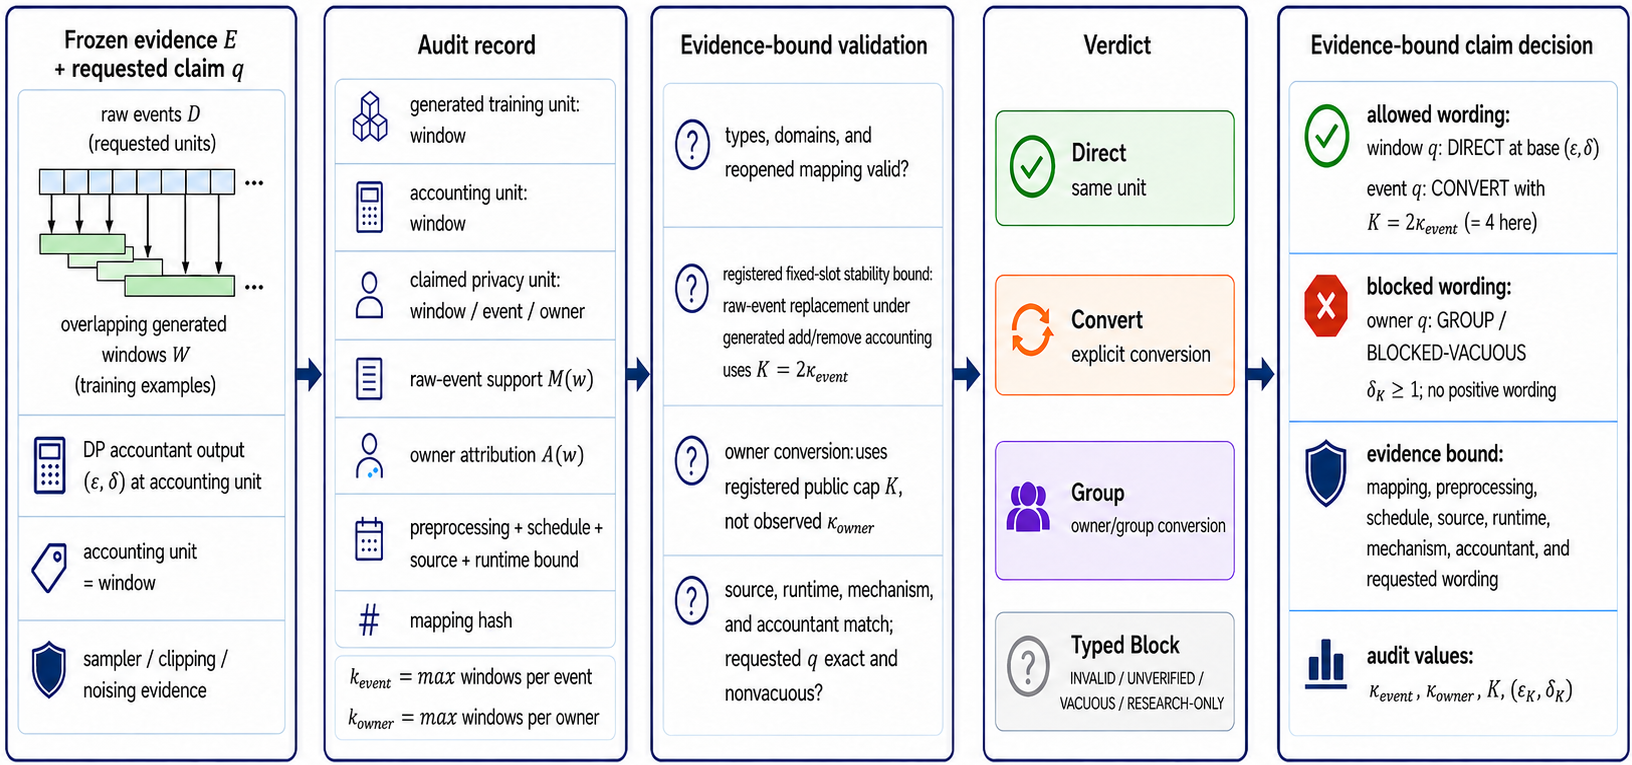
\includegraphics[width=\textwidth]{figures/ch02_source_evidence_validation.png}
    \caption{Evidence-bound validation and query separation for one frozen WISDM
    execution}
    \label{fig:ch2-evidence-validation-pipeline}
\end{figure}

\begin{lemma}[Query separation]
\label{lem:ch2-query-separation}
For fixed \(\EvidenceBundle\), suppose two requested claims satisfy
\(
\ClaimValidator(\EvidenceBundle,q_1)
\neq
\ClaimValidator(\EvidenceBundle,q_2)
\).
No query-oblivious interface \(A(\EvidenceBundle)\) can be exact for both
requests.
\end{lemma}

\begin{proof}[Proof]
The interface receives the same input for both requests and therefore has one
output distribution.  That distribution cannot be concentrated on two distinct
decision tuples.  Returning one common result is therefore incorrect for at least
one request; a common abstention is likewise inexact whenever either request is
licensed.  Hence exactness requires the requested claim to be supplied as an
input.
\end{proof}

Lemma~\ref{lem:ch2-query-separation} is an interface-separation result, not a new
privacy theorem.  It establishes why the query in
Equation~\eqref{eq:ch2-validator-decision} cannot be replaced by a display option
applied after an evidence-only verdict.  Figure~\ref{fig:ch2-evidence-validation-pipeline}
illustrates the consequence: one frozen execution can license two different
positive pairs and block a third sentence.  The next subsection specifies how a
registered distance \(K\) determines the converted pair and when the vacuity gate
forces \textsf{Blocked}.

\subsection{Privacy-Unit Conversion and Claim Blocking}
\label{subsec:privacy-unit-conversion}

Once the requested path has been identified, a conversion is licensed only by a
registered distance bound connecting the two adjacency relations.  Suppose the
bound execution is established as \((\varepsilon,\delta)\)-DP at generated-record
distance one and Equation~\eqref{eq:ch2-stability-bound} holds for an integer
\(K\geq1\).  Standard group privacy then gives

\begin{equation}
    \ConvertedEpsilon = K\varepsilon,
    \qquad
    \ConvertedDelta
    = \delta \sum_{i=0}^{K-1} e^{i\varepsilon}.
    \label{eq:ch2-group-conversion}
\end{equation}

Equation~\eqref{eq:ch2-group-conversion} is a registered consequence of the base
guarantee, not a new accountant or privacy theorem
\cite{dwork2014algorithmic}.  The validator neither estimates \(K\) from the
requested wording nor substitutes an observed incidence for a worst-case bound.
It first requires a registered transformation argument, then evaluates the
geometric sum with stable log-domain arithmetic.  For \(\varepsilon>0\), the
implementation uses

\begin{equation}
    \log \ConvertedDelta
    = \log\delta
    + \log\!\bigl(\operatorname{expm1}(K\varepsilon)\bigr)
    - \log\!\bigl(\operatorname{expm1}(\varepsilon)\bigr),
    \label{eq:ch2-stable-delta}
\end{equation}

with the exact \(\varepsilon=0\) limit \(\ConvertedDelta=K\delta\).  This avoids
overflow without changing the privacy consequence.  A public pair is emitted only
when both values are finite, \(\ConvertedEpsilon\geq0\), and
\(0<\ConvertedDelta<1\).  A non-finite result,
\(\ConvertedDelta\geq1\), or an unregistered derivation blocks positive wording.
The resulting values may remain visible as diagnostics, but their presence does
not convert a vacuous result into an allowed privacy claim; clamping delta to one
for serialization is not a privacy result.

\begin{proposition}[Contract-relative consequence]
\label{prop:ch2-contract-relative-consequence}
Assume that (i) \(\EvidenceBundle\) describes \(\DataTransform\) and the executed
mechanism \(\DPMechanism\); (ii) a registered checker establishes
\[
    \GeneratedAdjacencyMetric\!\left(
        \DataTransform(\RawDataset),
        \DataTransform(\RawDataset')
    \right) \leq K
\]
for every pair satisfying
\(\RawAdjacencyMetric(\RawDataset,\RawDataset')\leq1\); and (iii) a registered
accountant establishes \((\varepsilon,\delta)\)-DP for the bound execution at
generated-record distance one.  Then \(\DPMechanism\circ\DataTransform\) satisfies
Equation~\eqref{eq:ch2-group-conversion} for the requested raw adjacency.  If
\(K=1\) and the units and metrics coincide, the base pair takes the
\textsf{Direct} path.
\end{proposition}

\begin{proof}[Proof]
For a raw-adjacent pair, premise (ii) supplies a generated-metric path of length at
most \(K\) between the two transformed datasets.  Applying the distance-one DP
inequality successively along that path multiplies the likelihood factor by
\(e^{\varepsilon}\) at each step.  The additive terms accumulate with multipliers
\(1,e^{\varepsilon},\ldots,e^{(K-1)\varepsilon}\), which yields
Equation~\eqref{eq:ch2-group-conversion}.  When \(K=1\), the expression reduces to
the base pair.  The conclusion is conditional on the three registered premises;
the validator checks their disclosed evidence rather than proving execution
fidelity.
\end{proof}

The metric pair is essential when selecting \(K\).  A raw replacement can replace
several generated windows, but a replacement is one edit under a generated
replace-one metric and two edits under a generated add/remove metric.  This
distinction produces the factor-of-two case summarized in
Table~\ref{tab:ch2-adjacency-distance}.

\begin{corollary}[Factor-two mapping]
\label{cor:ch2-factor-two-mapping}
Assume public fixed-slot identities and a registered complete-support bound under
which one raw-event replacement changes at most \(\EventIncidence\) generated
records.  A generated add/remove accountant licenses
\(K=2\EventIncidence\), whereas a generated replace-one accountant licenses
\(K=\EventIncidence\).
\end{corollary}

\begin{proof}[Proof]
Each affected generated record is replaced.  Under add/remove distance, one such
replacement consists of one removal and one addition, so at most
\(2\EventIncidence\) edits are required.  Under replace-one distance, each
replacement costs one edit, giving \(\EventIncidence\).  The conclusion relies on
the registered complete-support premise; observed overlap alone is insufficient.
\end{proof}

These consequences produce four distinct decision cases.  A native-unit request
with coincident adjacency uses \(K=1\) and retains the base pair as
\textsf{Direct}.  A raw-event request takes \textsf{Convert} only when the event
stability argument and its metric-specific \(K\) are registered.  An owner request
takes \textsf{Group} when a public contribution bound supplies the generated
distance.  If no such bound is registered, the path is \textsf{Underspecified}; if
the bound exists but Equation~\eqref{eq:ch2-group-conversion} is non-finite or
vacuous, the path remains typed but the release is \textsf{Blocked}.

The WISDM evidence in Figure~\ref{fig:ch2-evidence-validation-pipeline}
illustrates why a public cap and an observed maximum are not interchangeable.  Its
fixed-slot event replacement has \(\EventIncidence=2\) and generated add/remove
accounting, so Corollary~\ref{cor:ch2-factor-two-mapping} gives \(K=4\).  For the
owner path, a public prefix policy caps contributions at 600 windows before
training.  The observed maximum of 565 verifies compliance with that policy but
does not replace it as a neighboring-dataset bound; the conversion therefore uses
\(K=600\).  Because the resulting \(\ConvertedDelta\) is at least one, the owner
path is reported as \textsf{Group}/\textsf{Blocked} and no positive owner-level
sentence is released.

The conversion rule thus determines what follows if the evidence premises hold;
it does not establish that the disclosed mapping, runtime, mechanism, and
accountant all belong to the same execution.  The next subsection specifies those
binding obligations and the assurance boundary of a bundle-only decision.

\subsection{Decision Procedure and Artifact Invalidation}
\label{subsec:evidence-binding-boundary}

The conversion consequence in Section~\ref{subsec:privacy-unit-conversion} is
meaningful only when the transformation, runtime, mechanism, and accountant
records refer to the same reported execution.  The validator therefore binds more
than a model artifact and a final privacy pair.  Its internal record includes the
selected mapping and identities; event support and owner attribution;
preprocessing, population, contribution, selection, and schedule policies;
mechanism, runtime, source, and accountant versions; base privacy parameters; and
the requested-unit contract.  The public view may redact private provenance, but
it retains the decision, artifact bindings, numerical result or diagnostic,
assumptions, forbidden wording, localized issues, and conditions that trigger
revalidation.

The finite-registry validator applies the following eight phases in order.  This
procedure is a typed evidence-to-wording decision, not a training algorithm.

\begin{enumerate}[label=(\arabic*),leftmargin=*,itemsep=3pt,topsep=4pt]
    \item \textbf{Types and domains.} Exact typed parsing rejects Boolean values
    supplied as integers, non-finite numerical values, invalid probabilities, and
    fields outside the registered domain before any privacy consequence is
    evaluated.

    \item \textbf{Reopened mapping.} The validator reopens the mapping rather than
    trusting a copied report string.  It recomputes file and semantic bindings,
    selected identities, intervals, event supports, owner attributions,
    \(\EventIncidence\), and \(\OwnerIncidence\).

    \item \textbf{Registered stability.} The selected checker must cover record
    identity and influence together with preprocessing, population, contribution,
    schedule, and selection dependencies.  A checker that covers only observed
    overlap does not establish Equation~\eqref{eq:ch2-stability-bound}.

    \item \textbf{Runtime agreement.} Observed fields must match the registered
    sampler, sampling rate, optimization steps, noise and clipping rules,
    accounting unit, mapping and pipeline identities, and secure-randomness mode.
    Missing runtime observation blocks concrete-run wording.

    \item \textbf{Registry binding.} A versioned registry binds supported source
    and adapter identities to the mechanism semantics and accountant.  The
    validator recomputes the base pair and default-denies unknown adapters,
    attachments, or accounting rules.

    \item \textbf{Path resolution.} The requested unit and adjacency select the
    direct, converted, grouped, or underspecified path and its registered
    stability method.  The validator never infers a path from the wording alone.

    \item \textbf{Numerical consequence.} The base pair is retained only on the
    exact native path.  Otherwise Equations~\eqref{eq:ch2-group-conversion}
    and~\eqref{eq:ch2-stable-delta} are evaluated under the registered \(K\).

    \item \textbf{Typed release.} Exact wording, issue precedence, the non-finite
    and vacuity gates, and the authority label determine the public report.  The
    operational metadata may be redacted without changing that decision.
\end{enumerate}

Four complementary digests support these checks.  A full-file digest detects byte
substitution.  A canonical selected digest binds the normalized semantic records
that participate in the run, so permutation or irrelevant decoy rows cannot
silently redefine the selected mapping.  A pipeline digest binds transformation
and policy parameters, and a runtime digest binds the observed mechanism fields.
These digests expose changed, stale, or mutually inconsistent artifacts.  They do
not establish that the producer executed the referenced bytes: equal mapping
digests do not prove sampler use, and equal report text cannot replace reopening
the underlying files.  Changing a bound mapping, selected identity, preprocessing
or population rule, contribution policy, schedule, mechanism or accountant
version, runtime parameter, claim unit, adjacency, or conversion method therefore
invalidates the old report and triggers validation again.  A redacted public view
is a view of the same decision, not a separately certified claim.

When several conditions apply, the implemented release precedence is

\begin{equation}
\begin{split}
    \textsf{Blocked-Invalid} &\;>\; \textsf{Blocked-Unverified}
    \;>\; \textsf{Blocked-Vacuous} \\
    &\;>\; \textsf{Research-Only} \;>\; \textsf{Allowed}.
\end{split}
\label{eq:ch2-release-precedence}
\end{equation}

The ordering prevents a valid scalar calculation from masking a malformed input
or missing runtime trace.  Likewise, an external attachment cannot repair an
unrelated mechanism contradiction, and a blocked internal diagnostic cannot be
converted into an allowed public sentence by redaction.

\subsection{Evidence Authority, Complexity, and Non-Attestation Boundary}
\label{subsec:ch2-evidence-authority}

The validation cost is dominated by reopening and checking these structures.  For
\(B\) mapping bytes, \(R\) rows, \(S\) selected rows, \(A\) attribution entries,
and \(P\leq2A\) interval endpoints, the registered checks require
\(O(B+R+A+S\log S+P\log P)\) time and \(O(R+A)\) memory, in addition to the work
of the registered accountant.  This bound describes the complete validator; a
specialized aggregate rescan that checks only mapping statistics is not an
equivalent certificate.

The remaining assurance boundary is informational.  A bundle-only validator can
test consistency among the objects it receives, but unauthenticated self-reporting
cannot distinguish faithful execution from a producer that presents the same
bundle after executing different code or hiding a dependency.

\begin{proposition}[Bundle-only non-attestation]
\label{prop:ch2-bundle-only-non-attestation}
Let a validator observe only an unauthenticated tuple
\((\EvidenceBundle,\ClaimQuery,\ValidationRegistry)\).  Suppose a faithful world
and a world that reports the same tuple while executing different code or hiding
a dependency are observationally identical to the validator.  Every deterministic
or randomized validator has the same output distribution in both worlds and
therefore cannot establish execution fidelity from that tuple alone.
\end{proposition}

\begin{proof}[Proof]
The validator receives identical inputs in the two worlds.  A deterministic
validator must consequently return the same output, and a randomized validator
must induce the same conditional output distribution.  No decision rule over the
observed tuple can separate the worlds without an additional authenticated
observation.
\end{proof}

The threat model is consequently an honest-but-fallible producer: stale exports,
omitted dependencies, inconsistent configuration, mismatched artifacts, and
unjustified privacy-unit restatement are in scope.  A malicious producer that can
fabricate a mutually consistent bundle while running another procedure is outside
the positive assurance claim.  Addressing that adversary requires authenticated
runtime observation, execution attestation, or a cryptographic proof system
\cite{narayan2015verifiable,shamsabadi2024confidential}.  The experiments in the
next section test whether the registered observable obligations separate designed
allowed and non-allow cases; they do not measure faithful execution.  In this
chapter, \textsf{EVIDENCE\_VALIDATED} means that registered observable obligations
pass; it does not mean execution fidelity.

\section{Experimental Evaluation}
\subsection{Controlled Validation and Ablation}
\label{subsec:controlled-validation-ablation}

The first experimental question is which claim distinctions disappear when the
validator observes only a weak projection of the evidence or when a registered
obligation is removed.  The controlled suite contains 100 allowed cases spanning
five registered path strata---direct window, direct event, direct owner,
converted event, and grouped owner---at five boundary or scale levels and in four
mapping contexts.  The contexts include a canonical mapping, irregular supports,
non-selected decoy rows, and permuted file order.  Each allowed parent is paired
with one non-allow case.  The 100 paired cases are produced by 25 one-premise
mutation operators, each applied to four distinct parents, so that every allowed
parent is consumed once.

An authored manifest, rather than the output of the full validator, declares the
expected path, release and assurance state, localized issue, and numerical rule.
Every method receives the same report, audit row, and mapping.  The
\emph{unsafe-positive fraction} is the fraction of the 100 non-allow cases that
nevertheless receive an allowed decision.  The \emph{valid-exact fraction} is the
fraction of the 100 allowed cases for which both the decision path and privacy
pair are exact.  The \emph{exact-tuple fraction} is evaluated over all 200 cases
and additionally requires the correct assurance state, block subtype, and
presence or absence of numerical output.  These fractions are deterministic
coverage outcomes for the authored suite.  They are neither estimates of a
deployment population nor empirical error rates.

Table~\ref{tab:ch2-controlled-ablation} compares the complete registered contract
(\textsf{FULL}) with two kinds of deliberately weakened checks.  B0--B4 are
information projections that retain only field presence, JSON Schema validity,
multiplicity, mapping-hash binding, or base-accountant recomputation.  A1 leaves
the static contract intact but assumes that runtime evidence matches it, whereas
A2 removes only the vacuity gate.  The rows are therefore diagnostic projections
and obligation ablations, not predecessor systems or competing validators.

\begin{table}[tbp]
    \centering
    \caption{Controlled-suite and ablation results}
    \label{tab:ch2-controlled-ablation}
    \footnotesize
    \setlength{\tabcolsep}{2.3pt}
    \renewcommand{\arraystretch}{1.13}
    \begin{tabular}{@{}
        >{\raggedright\arraybackslash}p{0.19\textwidth}
        >{\centering\arraybackslash}p{0.105\textwidth}
        >{\centering\arraybackslash}p{0.105\textwidth}
        >{\centering\arraybackslash}p{0.105\textwidth}
        >{\raggedright\arraybackslash}p{0.31\textwidth}@{}}
        \toprule
        \textbf{Probe / full contract} &
        \textbf{Unsafe-positive frac.} &
        \textbf{Valid-exact frac.} &
        \textbf{Exact-tuple frac.} &
        \textbf{Principal evidence not checked} \\
        \midrule
        B0 Field presence &
        1.00 & 0.60 & 0.00 &
        types, semantics, files, execution, accounting \\

        B1 JSON Schema &
        0.96 & 0.60 & 0.00 &
        cross-field and execution semantics \\

        B2 Multiplicity only &
        1.00 & 0.80 & 0.00 &
        stability/adjacency, staleness, mechanism \\

        B3 Hash only &
        0.96 & 0.60 & 0.00 &
        consistently wrong semantics or mechanism \\

        B4 Accountant only &
        0.88 & 0.60 & 0.00 &
        mapping, claimed unit, dependencies, runtime \\

        A1 Runtime assumed matched &
        0.12 & 1.00 & 0.94 &
        independent runtime/artifact equality \\

        A2 \textsf{FULL} minus vacuity &
        0.04 & 1.00 & 0.98 &
        reportability of converted numerics \\

        \textsf{FULL} &
        \textbf{0.00} & \textbf{1.00} & \textbf{1.00} &
        registered-contract assurance boundary \\
        \bottomrule
    \end{tabular}
\end{table}

The complete contract produces no unsafe positive among the 100 paired
non-allow cases, exactly matches all 100 allowed cases, and returns the expected
full tuple in all 200 cases.  An independent standard-library implementation of
the grid and mutation oracle passes 20,909 of 20,909 checks, and the expanded
contract suite passes 83 of 83 checks.  These checks establish conformance to the
finite authored contract, not correctness for an unregistered mechanism or
unobserved execution.

The weaker rows expose distinct losses of information.  B0, B1, B3, and B4 reuse
the base privacy pair in 40 allowed conversion or grouping cases, while B2 does so
in four.  A1 retains every allowed case but leaves 12 unsafe positives: four each
for missing-trace, runtime-noise, and runtime-artifact mutations.  A2 leaves four
vacuous owner-level positives.  Five fixed necessity witnesses isolate the
corresponding obligations: reopened mapping bytes, registered stability status,
runtime noise and trace equality, the vacuity gate, and exact event rather than
window wording.  Removing each obligation erases the decision boundary between
its paired valid and blocked witness.  Independent recomputation passes all 10
witness decisions as well as their associated tamper tests.

\begin{table}[tbp]
    \centering
    \caption{Fixed information-necessity witnesses}
    \label{tab:ch2-necessity-witnesses}
    \footnotesize
    \setlength{\tabcolsep}{2.8pt}
    \renewcommand{\arraystretch}{1.13}
    \begin{tabular}{@{}
        >{\centering\arraybackslash}p{0.07\textwidth}
        >{\raggedright\arraybackslash}p{0.26\textwidth}
        >{\raggedright\arraybackslash}p{0.27\textwidth}
        >{\raggedright\arraybackslash}p{0.30\textwidth}@{}}
        \toprule
        \textbf{ID} & \textbf{Fixed comparison} &
        \textbf{Deleted or hidden edge} & \textbf{Required distinction} \\
        \midrule
        W1 & Valid parent P01 vs. blocked F02 &
        Actual mapping bytes; report, audit row, and query held equal &
        \textsf{Allowed} vs. \textsf{Blocked-Invalid} \\

        W2 & Converted parent P02 vs. F16 &
        Registered stability status; remaining public fields held equal &
        \textsf{Convert/Allowed} vs. \textsf{Blocked-Unverified} \\

        W3 & Direct parent P01 vs. F05 &
        Runtime noise and trace equality &
        \textsf{Direct/Allowed} vs. \textsf{Blocked-Invalid} \\

        W4 & F01 under A2 vs. \textsf{FULL} &
        Vacuity and reportability gate &
        Unsafe owner positive vs. typed vacuous block \\

        W5 & One WISDM event certificate &
        Exact licensed event sentence replaced by a valid window sentence &
        Independent wording verifier rejects the substitution \\
        \bottomrule
    \end{tabular}
\end{table}

Table~\ref{tab:ch2-necessity-witnesses} is intentionally narrower than a universal
minimality claim.  The witnesses show that deleting one named edge loses a
required distinction on authenticated fixed inputs; they do not prove that every
audit engine must use the same files or that such failures occur at a measured
rate in published systems.

A second authority source avoids relying only on newly authored mutations.  A
protocol fixed before the conformance construction identified ten preserved
development incidents whose root causes affected claim-bearing output and had
pre-protocol discovery records.  A production-import-free verifier reopens the
historical source or archive member, discovery anchor, consequence, and 16 repaired
controls, passing 176 of 176 checks.  Three tamper tests retain the authentic
lineage and reject an omitted incident or forged archive identity.  This is actual
development lineage from the evaluated system, but it is not an independently
sampled publication corpus and therefore does not estimate real-world prevalence.

For scope comparison, the official TensorFlow Privacy 0.9.0 privacy-statement
function \cite{google2024tfprivacy} is evaluated on the original 23-case subset
that can be expressed through its scalar interface.  Given caller-supplied
scalars and a group bound, it returns finite conditional statements for all seven
valid cases and for 15 of 16 non-allow bundles; it rejects a Boolean value supplied
for the number of steps.  All 79 reproduction checks re-execute and hash the
official module and setup.  In the fixed-base vacuity case, the function solves a
smaller example-level delta and freshly targets a user-level delta.  This is a
useful alternative accounting contract, but it is not
Equation~\eqref{eq:ch2-group-conversion} applied to the supplied privacy pair.
Accordingly, the comparison is not a quality ranking: the scalar function derives
a conditional statement from values supplied by its caller, whereas
\textsf{FULL} reopens the pipeline evidence and decides whether the exact
submitted tuple supports the requested sentence.  The next subsection tests that
evidence-bound distinction on activity data and mapping-only rescans.

\subsection{Complete Activity-Data Executions}
\label{subsec:activity-mapping-validation}

The second experimental question asks whether one frozen evidence bundle produces
distinct query-dependent decisions and whether that pattern recurs across fresh,
separately bound executions.  The complete activity-data path uses the public
WISDM accelerometer data \cite{kwapisz2011activity}.  A public parser reduces
1,098,210 physical lines to 1,086,465 canonical valid events.  From these events,
the registered transformation constructs 7,304 training windows, each with length
200 and stride 100.  Owner identities partition the mapping, feature and label transforms
are record-local, and a public prefix policy caps training-window contributions at
600 per owner before training.  The bound run uses Poisson window sampling at
\(1/50\), 100 optimization steps, and noise multiplier 2.  Registered RDP
recomputation yields the base pair
\((0.536827391167,10^{-6})\).

Every request in Table~\ref{tab:ch2-wisdm-query-decisions} reopens the same
7,304-row mapping and binds the same pipeline and runtime evidence.  The window
query is native to the accountant and therefore uses \(K=1\).  Under fixed-slot
raw-event replacement, the reopened mapping gives
\(\EventIncidence=2\); because the base metric is generated add/remove,
Corollary~\ref{cor:ch2-factor-two-mapping} gives \(K=4\).  The owner request
observes a maximum contribution of 565 only as a compliance check.  Its registered
conversion uses the public cap \(K=600\), not that observed maximum.

\begin{table}[tbp]
    \centering
    \caption{Query-dependent decisions for one frozen WISDM execution}
    \label{tab:ch2-wisdm-query-decisions}
    \small
    \setlength{\tabcolsep}{3pt}
    \renewcommand{\arraystretch}{1.15}
    \begin{tabular}{@{}
        >{\raggedright\arraybackslash}p{0.17\textwidth}
        >{\centering\arraybackslash}p{0.17\textwidth}
        >{\raggedright\arraybackslash}p{0.23\textwidth}
        >{\raggedright\arraybackslash}p{0.29\textwidth}@{}}
        \toprule
        \textbf{Requested claim} &
        \textbf{Observed / registered (K)} &
        \textbf{Path / release} &
        \textbf{Pair or action} \\
        \midrule
        Window &
        -- / 1 &
        \textsf{Direct} / \textsf{Allowed} &
        \((0.53683,10^{-6})\) \\

        Raw event &
        2 / 4 &
        \textsf{Convert} / \textsf{Allowed} &
        \((2.14731,1.0642\times10^{-5})\) \\

        Owner &
        565 / 600 &
        \textsf{Group} / \textsf{Blocked} &
        vacuous: \(\delta_K\geq1\) \\
        \bottomrule
    \end{tabular}
\end{table}

Thus the same execution licenses the base window sentence, licenses a weaker
event-level sentence after registered conversion, and withholds positive
owner-level wording.  The owner path remains \textsf{Group}; its release is
separately \textsf{Blocked} because Equation~\eqref{eq:ch2-group-conversion}
produces \(\varepsilon_K=322.096\).  Its converted delta satisfies
\(\log_{10}\delta_K=134.033097\), and hence \(\delta_K\geq1\).  The existence of those
diagnostic numbers does not make them reportable privacy parameters.

Five post-freeze WISDM runs have distinct model digests and preserve all three
decision paths and privacy values.  Across those runs, accuracy is
\(0.6556\pm0.0080\) and macro-F1 is \(0.3922\pm0.0033\).  A separately bound
The complete pipeline---raw parsing, mapping, training, report generation, and
evidence production---takes \(16.743\pm1.191\) seconds over the five runs in the
reported environment.  Independent verification with raw reconstruction takes
\(6.480\pm0.428\) seconds.  Five additional portable invocations take
\(1.577\pm0.125\) seconds and pass 35 of 35 checks each while omitting the three
raw-input reconstruction checks.  A complete run directory averages 0.996 MB;
the separately acquired 50.326 MB raw file is required only for full-source
reconstruction.  These end-to-end timings include process startup and are not
isolated validator overhead.

A separately bound route uses the UCI Human Activity Recognition Using Smartphones data
\cite{anguita2013har,reyesortiz2013uci}, with 7,352 training windows, 2,947 test
windows, and 561 features.  Each of five post-freeze runs passes 49 of 49
raw-source checks and 38 of 38 portable checks with a distinct digest.  Because
event support and an owner contract are absent, each run licenses only
\textsf{Direct} window add/remove wording at approximately
\((0.536827,10^{-6})\); event and owner requests are blocked rather than inferred.
Its mean accuracy is \(0.8049\pm0.0315\), and mean macro-F1 is
\(0.7795\pm0.0504\).  Both datasets' accuracy and F1 values are integration
diagnostics, not competitive or state-of-the-art utility claims.

\begin{table}[H]
    \centering
    \caption{Invariant UCI HAR authorization boundary across five executions}
    \label{tab:ch2-uci-authorization}
    \small
    \setlength{\tabcolsep}{5pt}
    \renewcommand{\arraystretch}{1.15}
    \begin{tabular}{@{}
        >{\raggedright\arraybackslash}p{0.20\textwidth}
        >{\centering\arraybackslash}p{0.22\textwidth}
        >{\centering\arraybackslash}p{0.22\textwidth}
        >{\centering\arraybackslash}p{0.12\textwidth}@{}}
        \toprule
        \textbf{Requested unit} & \textbf{Release status} &
        \textbf{Path} & \textbf{\(K\)} \\
        \midrule
        Published window & \textsf{Allowed} & \textsf{Direct} & 1 \\
        Raw event & \textsf{Blocked-Unverified} & \textsf{Underspecified} & -- \\
        Owner & \textsf{Blocked-Unverified} & \textsf{Underspecified} & -- \\
        \bottomrule
    \end{tabular}
\end{table}

Table~\ref{tab:ch2-uci-authorization} is invariant across all five protocol-fixed
runs.  This negative result is informative: an existing published-window dataset
does not automatically expose the raw-session support or public owner cap needed
for a stronger unit claim, even when the DP-SGD mechanism and accountant are
otherwise reproduced.

\subsection{Sepsis and Backblaze Mapping Diagnostics}
\label{subsec:ch2-mapping-diagnostics}

The third experimental question isolates the transformation side of the contract
at substantially larger scales.  For
the PhysioNet/Computing in Cardiology 2019 Sepsis data
\cite{goldberger2000physiobank,reyna2019sepsis,reyna2020sepsis}, the verifier
opens and hashes 5,000 patient files and reconstructs 16 mappings under dense,
non-overlap, and public-cap policies.  For the Backblaze first-quarter 2025 drive
statistics \cite{backblaze2025stats}, a verifier without production imports
rescans 1.02 GB comprising 90 daily files, 27,799,986 drive-day rows, and 318,426
drives.  It distinguishes windows over ordered available snapshots, which may
compress calendar gaps, from calendar-contiguous windows.

The Sepsis source contains 192,206 hourly patient rows.  Six-, twelve-, and
twenty-four-hour window policies cover dense, half-stride, and non-overlap
schedules, while public owner-local prefix caps of 1, 4, 8, and 16 make the
contribution rule observable before selection.  Label-balanced caps act as
negative controls: they can reproduce the same displayed counts as a public
prefix cap while using private labels to change selected identities.  Candidate
event distance is therefore reported only for fixed positional or public-prefix
policies whose support premise is registered.

The Backblaze rescan covers 27,799,986 unique drive-day events with no duplicate
serial-number and date pair and evaluates 22 mapping policies.  Ordered-snapshot and
calendar-contiguous windows can display equal incidence while selecting different
records; public owner-prefix caps are evaluated separately.  This distinction is
why a compact table can summarize representative rows but cannot replace the full
policy identity bound into the mapping evidence.

\begin{table}[tbp]
    \centering
    \caption{Mapping-only diagnostics for Sepsis and Backblaze data}
    \label{tab:ch2-mapping-only-diagnostics}
    \footnotesize
    \setlength{\tabcolsep}{2.8pt}
    \renewcommand{\arraystretch}{1.12}
    \begin{tabular}{@{}
        >{\raggedright\arraybackslash}p{0.10\textwidth}
        >{\raggedright\arraybackslash}p{0.29\textwidth}
        >{\raggedleft\arraybackslash}p{0.14\textwidth}
        >{\centering\arraybackslash}p{0.09\textwidth}
        >{\centering\arraybackslash}p{0.11\textwidth}
        >{\centering\arraybackslash}p{0.09\textwidth}@{}}
        \toprule
        \textbf{Dataset} &
        \textbf{Mapping policy} &
        \textbf{Generated records} &
        \textbf{Obs. \(\EventIncidence\)} &
        \textbf{Candidate event \(K\)} &
        \textbf{Obs. \(\OwnerIncidence\)} \\
        \midrule
        Sepsis & 6h dense & 167,206 & 6 & 12 & 331 \\
        Sepsis & 6h non-overlap & 29,958 & 1 & 2 & 56 \\
        Sepsis & public owner cap 1 & 5,000 & 1 & 2 & 1 \\
        \midrule
        Backblaze & 7d dense, ordered snapshots & 25,904,370 & 7 & 14 & 84 \\
        Backblaze & 7d dense, calendar-contiguous & 25,867,949 & 7 & 14 & 84 \\
        Backblaze & 7d non-overlap, ordered & 3,709,484 & 1 & 2 & 12 \\
        Backblaze & 7d non-overlap, calendar & 3,707,669 & 1 & 2 & 12 \\
        Backblaze & 60d non-overlap, ordered & 304,906 & 1 & 2 & 1 \\
        Backblaze & 60d non-overlap, calendar & 302,760 & 1 & 2 & 1 \\
        \bottomrule
    \end{tabular}
\end{table}

The Sepsis and Backblaze verifiers pass 128 of 128 and 86 of 86 checks,
respectively.  Table~\ref{tab:ch2-mapping-only-diagnostics} nevertheless exposes
three distinct premise risks.  First, non-overlap can reduce
\(\EventIncidence\) to one while fixed-slot replacement under generated
add/remove accounting still gives candidate \(K=2\).  Second, ordered and
calendar-contiguous Backblaze semantics differ by 36,421 dense seven-day windows
despite equal incidence.  Third, a Sepsis label-balanced selection can reproduce
public-cap counts while privately changing selected identities.  The rescans
reconstruct rows and policies, but neither bundle binds a mechanism, runtime, or
accountant.  Consequently, every row is only a mapping diagnostic: no row is an
\((\varepsilon,\delta)\) certificate or a \textsf{Direct} verdict, and no positive
privacy wording is emitted.

\subsection{Independent Verification, External Intake, and Reproducibility}
\label{subsec:ch2-independent-verification}

The final experimental question asks whether each result can be reconstructed
without merely importing the production validator.  Separate implementations
reopen the relevant inputs, recompute hashes, rows, decisions, and numerical
tolerances, and confirm that a blocked public output contains no positive
sentence.  Table~\ref{tab:ch2-verification-surfaces} reports the principal
surfaces.  The denominators enumerate deterministic assertions in fixed artifacts;
they are not confidence intervals or independent human replications.

\begin{table}[tbp]
    \centering
    \caption{Independent verification surfaces and stated authority}
    \label{tab:ch2-verification-surfaces}
    \footnotesize
    \setlength{\tabcolsep}{3pt}
    \renewcommand{\arraystretch}{1.13}
    \begin{tabular}{@{}
        >{\raggedright\arraybackslash}p{0.34\textwidth}
        >{\centering\arraybackslash}p{0.18\textwidth}
        >{\raggedright\arraybackslash}p{0.37\textwidth}@{}}
        \toprule
        \textbf{Surface} & \textbf{Passing checks} &
        \textbf{Authority} \\
        \midrule
        Expanded contract regression & 83/83 &
        Fixed schema, registry, and release semantics \\
        Designed 200-case conformance surface & 20,909/20,909 &
        Five strata, 25 operators, fixed oracle and lineage \\
        Necessity witnesses & 10/10 &
        Five fixed edge-deletion distinctions \\
        Retrospective development lineage & 176/176 &
        Ten preserved incidents and 16 repaired controls \\
        TensorFlow Privacy scope comparison & 79/79 &
        Re-execution and hashing of the official scalar interface \\
        WISDM reference and each confirmatory run & 38/38 &
        Full raw reconstruction and three query decisions \\
        UCI HAR full / portable, each run & 49/49 / 38/38 &
        Published-input reconstruction / distributable evidence \\
        Sepsis / Backblaze mapping rescans & 128/128 / 86/86 &
        Mapping and policy diagnostics only \\
        \bottomrule
    \end{tabular}
\end{table}

An externally authored ExtraSensory source-path intake provides a separate
authority test \cite{loya2022extrasensory,vaizman2017context}.  Six terminal
records are retained rather than reporting only the successful attempt: repository
import, path, disk, loader, and plotting failures precede one complete five-epoch
execution.  The final run produces all 17 expected outputs, and separate verifiers
reconstruct its mapping and execution records.  Nevertheless, the external source
sets \texttt{secure\_rng=False} and prints a configured target epsilon rather than
an accountant-derived achieved epsilon.  The terminal result is therefore
execution-complete but claim-unverified; positive DP wording remains empty.  This
case demonstrates why successful training and artifact presence are not sufficient
authority for a privacy sentence.

The reproducibility package pins the core Python dependencies, schemas, registry,
claim-bearing reports, frozen outputs, and verification entry points.  Every
reported table row has a machine-readable source, while larger public datasets are
identified by acquisition boundary and digest rather than redistributed.  Exact
frozen-number verification does not require retraining; fresh WISDM runs use new
private randomness, so the verifier requires internal consistency and invariant
decision semantics rather than identical model or batch-trace hashes.  No
nondeterministic outcome is silently dropped, and missing raw inputs, unregistered
adapters, research randomness, private-dependent selection, and vacuous conversion
remain typed limitations rather than being converted into positive results.

\section{Summary}
\label{sec:ch2-summary-transition}

This chapter treated a privacy statement as a query over frozen execution
evidence rather than as a synonym for an accountant output.  The validator first
checks whether the requested unit and adjacency are connected to the generated
records, mechanism, runtime, and accountant through a registered evidence chain.
It then reports a typed path and independently decides whether positive wording is
allowed.  As a result, one completed execution can support a native-unit claim,
support a weaker converted claim, and block a stronger claim without collapsing
those outcomes into one privacy label.

The resulting assurance is deliberately bounded.  It is relative to the supplied
evidence and a finite validation registry; it is not execution attestation, an
arbitrary-code proof, or a new accountant.  Reopened artifacts, semantic digests,
runtime equality, registered stability, recomputation, and fail-closed release
reduce accidental claim--evidence mismatches under the honest-but-fallible threat
model.  They cannot distinguish faithful execution from a producer that presents
a consistently fabricated bundle.  Missing, unregistered, non-finite, or vacuous
premises therefore suppress positive wording rather than justify extrapolation.

The practical conclusion is a reuse boundary.  A completed model may be reused
with the exact native or converted wording licensed by its evidence, but a blocked
patient- or owner-level request cannot inherit the window-level pair.  Satisfying
that stronger request requires additional registered premises or a new mechanism
and execution native to the requested unit.  Chapter~\ref{ch:pp-mark} turns from
privacy wording to generative-image provenance.  The assurance object changes,
but the same dissertation-level question remains: whether a public decision is
supported by the target, mechanism, interface, and evidence that the decision
claims to represent.

\chapter[Secure Public Verification of Generative-AI Provenance]{Secure Public Verification of Generative-AI Provenance: PP-Mark}
\label{ch:pp-mark}

\section{Introduction}
\label{sec:ch4-introduction}

The preceding two chapters developed the \AuditablePrivacy{} axis of this
dissertation.  They asked whether a privacy sentence is licensed by a completed
execution and whether a requested privacy route is coherently assembled before
that execution begins.  This chapter turns to a separate trust claim: whether a
third party can verify that a generated image is accompanied by evidence
consistent with a declared generation context.  The protected object, mechanism,
and evidence are different, but the assurance problem has the same form.  A
positive label should not be released merely because one observable statistic
crosses a threshold; the label must remain aligned with the process and evidence
that give it meaning.

Image provenance has become harder to establish as generative models have
improved.  Synthetic images can support benign creation, accessibility, and
simulation, but they can also be used for impersonation and misleading media.
The resulting provenance problem is not solved by visual inspection
alone~\cite{chesney2019deepfakes,longpre2024provenance}.  Content credentials and
signed metadata provide an important publication layer, yet the strength of a
provenance claim still depends on what the attached technical evidence actually
establishes~\cite{c2pa2026spec}.  A signature can authenticate a manifest supplied
by a key holder.  It does not, by itself, show that a registered watermark signal
was embedded according to the process named in that manifest.

Digital watermarking addresses this gap by placing a recoverable signal in the
image or in the generative process.  Post-hoc methods encode a message after an
image is produced, while latent and model-integrated methods introduce structured
signals during generation~\cite{zhu2018hidden,tancik2020stegastamp,
wen2023treerings,fernandez2023stablesignature}.  Verification commonly evaluates a
detector $D(I,\mathrm{md})$ and accepts when its score exceeds a calibrated
threshold.  This design offers low latency and can remain useful after moderate
compression or transformation.  Its weakness is also structural: once the
detector is public, the same decision surface that enables independent checking
becomes a target for queries, surrogate construction, or gradient-based
optimization~\cite{jiang2023evading,muller2025blackbox,lin2025crack}.

Keeping the detector private behind an application programming interface reduces
direct exposure but replaces technical verification with organizational trust.
Only the service operator can execute the hidden rule, rate-limit queries, or
resolve disputes.  A user cannot reproduce the judgment independently, and a
long-lived provenance record remains dependent on the continued availability and
integrity of one verifier.  Public verification and forgery resistance therefore
appear to pull in opposite directions: opening the detector improves auditability
but expands the attack surface, whereas closing it reduces independent
auditability.

This chapter studies \PPMark{}, a construction that changes the acceptance rule
rather than merely hiding or hardening the score.  The generator derives a latent
watermark from a secret-keyed binding to the prompt, seed, model identifier, and
resolution.  It commits a deterministic sample of the embedding trace under a
Merkle root and produces an SP1 zero-knowledge proof receipt.  A public verifier
recovers a statistical watermark score from the submitted image and verifies the
receipt against the declared context, the committed trace, and the exact
canonical image hash.  Full acceptance requires both conditions:

\begin{equation}
\begin{aligned}
    &\mathsf{PPMark}_{\mathrm{accept}}(I,\mathrm{md},\PPReceipt)=1\\
    &\quad\Longleftrightarrow
    \bigl(\PPDetectionScore(I,\mathrm{md})\geq\PPThreshold\bigr)
    \land
    \bigl(\mathsf{VerifyReceipt}(\PPReceipt;\PPPublicStatement)=1\bigr).
\end{aligned}
\label{eq:ch4-intro-accept}
\end{equation}

Equation~\eqref{eq:ch4-intro-accept} is the chapter's central claim-alignment
boundary.  The score provides image-side evidence that the expected signal is
recoverable.  The receipt provides process-side evidence that the opened committed
trace is consistent with a secret-key-derived binding and an image-bound challenge.
Neither term is promoted into the other.  A high score alone is a screening
result, not publicly verified provenance, and a valid receipt alone does not show
that the published pixels retain the detectable signal.

The contributions of this chapter are summarized as follows.

\begin{itemize}
    \item It formulates secure public provenance verification as a conjunctive
    evidence decision.  The public detector remains available for low-latency
    screening, while a stronger acceptance mode additionally requires a
    cryptographic receipt bound to the declared generation context and exact
    image.

    \item It defines a context-bound latent watermark.  A secret-keyed binding
    determines a Reed--Solomon payload, sampled latent positions, Gaussian
    baselines, and signed perturbations.  The same binding therefore anchors the
    statistical sign pattern and the proof predicate.

    \item It commits sampled trace tuples and verifies a randomized opening in an
    SP1 zkVM.  The construction states the public/private split explicitly and
    gives a conditional unforgeability bound containing hash, proof-system, and
    partial-opening failure terms.

    \item It evaluates the two verification modes against fabricated bindings,
    compliance bypass, black-box imprint transfer, white-box optimization,
    regeneration, steganalysis, and common image transformations.  It also records
    the proving, verification, receipt-size, quality, and two-model limits
    needed to interpret the result operationally.
\end{itemize}

The assurance boundary is deliberately narrower than proof of image truth or
authorship.  \PPMark{} does not determine whether the prompt is factually correct,
whether the depicted event occurred, whether a person owns a legal identity, or
whether every diffusion operation was faithfully executed.  Its circuit does not
re-simulate the full diffusion model.  It verifies the declared composite relation
over a committed sampled trace, and full acceptance is meaningful only under the
stated hash, proof-system, key-secrecy, predicate, statistical, and partial-opening
assumptions.  The correct conclusion is therefore that an accepted image carries
verifiable provenance evidence relative to the declared binding, not that the
image is unconditionally authentic.

\section{Background and Related Work}
\label{sec:ch4-background}

\subsection{Generative Image Watermarking and Provenance}
\label{subsec:ch4-watermark-background}

An image-watermarking system normally exposes three logical procedures.  An
embedding procedure receives an image or generation state and a payload; an
extraction procedure recovers a message or statistic from a candidate image; and a
decision procedure compares the recovered object with a reference or threshold.
These procedures can be placed at different points in the image pipeline.

Post-hoc watermarking changes the completed pixel image.  HiDDeN learns an
encoder--decoder pair for hiding data in images, StegaStamp targets robustness
under physical and geometric transformations, and more recent systems such as
TrustMark and InvisMark improve capacity or robustness at arbitrary image
resolutions~\cite{zhu2018hidden,tancik2020stegastamp,bui2025trustmark,
xu2025invismark}.  Post-hoc deployment is attractive because it can wrap an
existing generator.  At the same time, the watermark is separated from the
internal generation path and may be attenuated by regeneration or model-based
removal~\cite{zhao2024removable}.

Generative or semantic watermarking moves the signal into the model or latent
trajectory.  Tree-Ring introduces structured patterns in initial diffusion noise,
Gaussian Shading encodes a lossless latent distribution, and Stable Signature
roots a watermark in a latent-diffusion decoder~\cite{wen2023treerings,
yang2024gaussianshading,fernandez2023stablesignature}.  RingID extends ring-based
signals to multi-key identification, while WIND separates watermark detection into
two stages for public use~\cite{ci2024ringid,arabi2025wind}.  These methods differ
in payload, perceptual objective, and robustness profile, but their common public
interface is still usually a detector score or decoded identity.

Provenance requires a more precise interpretation than watermark presence.  A
positive score means that the submitted image resembles the detector's expected
signal strongly enough under a calibration rule.  It does not necessarily bind
that signal to one prompt, seed, model, resolution, or committed execution trace.
Likewise, signed content credentials authenticate the signed assertions and their
chain, but the assertion is only as strong as the evidence placed behind it.  The
technical question in this chapter is consequently not whether statistical
watermarks or signed manifests should be discarded.  It is how a public
watermark decision can be coupled to a separately checkable relation describing
the claimed generation context.

This distinction yields two complementary service levels.  A statistical mode can
scan large volumes of transformed images and tolerate small signal degradation.  A
proof-bearing mode can make a stronger statement about an exact published object,
but must carry an explicit proof artifact and generally rejects altered pixels.
Treating these modes as interchangeable would obscure both their value and their
limits.

\subsection{Forgery Vulnerabilities of Public Detectors}
\label{subsec:ch4-public-detector-forgery}

A removal attack begins with a watermarked image and tries to lower its detection
score while preserving acceptable image quality.  A forgery attack begins with an
unmarked or differently marked image and tries to raise the score associated with
a target source.  These goals are asymmetric.  Robustness against removal does not
imply resistance to forgery, because a highly stable but publicly exposed pattern
may be easy to implant in unrelated content.

Black-box imprint attacks demonstrate this distinction.  From a watermarked
reference, the adversary estimates a transferable imprint and optimizes an
arbitrary cover image so that a target detector attributes it to the reference
source~\cite{muller2025blackbox}.  The attack does not require disclosure of the
target scheme's internal key derivation.  Query access, proxy models, and common
latent structure can supply a useful optimization signal.  A successful attack
therefore produces a positive detector outcome without the generation process
that the verifier may implicitly associate with that outcome.

The white-box case is stronger.  When the detector or a differentiable surrogate
is public, an adversary can maximize the verification statistic directly under a
pixel perturbation budget.  Prior work shows that watermark-based detectors can be
evaded or optimized against when their decision rules are exposed, and public
knowledge of a watermark's structure can enable specialized removal
strategies~\cite{jiang2023evading,lin2025crack}.  Rate limits may slow a pure
query attack, but they do not create cryptographic evidence that a positive score
originated from the registered embedder.

A signature-only construction addresses a different object.  If metadata is
signed, an adversary without the signing key cannot alter it undetectably.  If the
signing key is available to a malicious producer or compromised operator,
however, the attacker can sign a fabricated binding or a clean image.  Adding a
score blocks the clean-image case only when the attacker cannot search for a
binding whose derived pattern happens to correlate with the image.  The resulting
problem is a claim--evidence mismatch: the public interface says ``verified,'' but
the evidence may show only that some chosen detector statistic crossed a threshold
and some metadata was signed.

The threat model used here grants the adversary watermarked images and all public
artifacts.  The adversary may manipulate pixels, query the public score, and use
detector gradients.  The PP-Mark binding key \PPSecretKey{} is not disclosed, and
the adversary is assumed unable to violate SHA-256 collision resistance or SP1
computational soundness.  A conventional metadata-signing key used in comparison
architectures is separate from \PPSecretKey{}; compromising that comparison key
does not reveal the PP-Mark binding key.  Conversely, compromise of
\PPSecretKey{} is an explicit failure of the operational assumption and is not
hidden by the theorem.

\subsection{Zero-Knowledge Proofs and Verifiable Computation}
\label{subsec:ch4-zkp-background}

Commit-and-open protocols allow a prover to fix a large object before learning
which parts a verifier will inspect.  A Merkle tree reduces the committed object
to one root; an authentication path then proves that an opened leaf belongs to the
committed tree without publishing every leaf~\cite{merkle1988signature}.  If the
opening challenge is derived after the commitment and is bound to the submitted
image, a prover cannot freely reuse one favorable opening for a different image.
The residual risk is explicit: a random opening can miss all positions at which a
committed trace cheats.  That probability becomes a term in the guarantee rather
than an implicit trust assumption.

Zero-knowledge proofs add a second property.  A prover can demonstrate that a
private witness satisfies a public predicate without revealing the witness itself.
PP-Mark realizes this layer with the SP1 zero-knowledge virtual machine, which can
prove execution of a Rust program and publish a standalone receipt~\cite{roy2024sp1}.
The proof program checks key binding, Merkle commitment, image-bound challenge,
and deterministic embedding relations.  It does not prove the semantic truth of
the context fields, and it does not re-run the complete image generator.

Related provenance systems occupy adjacent points in this design space.  C2PA
standardizes signed content credentials and manifest relationships, whereas
PP-Mark supplies evidence about a watermark embedding relation that can be carried
with such metadata~\cite{c2pa2026spec}.  VeriLLM uses commitment and randomized
opening to make decentralized inference publicly checkable; PP-Mark applies a
related commit--open--verify idea to sampled image-watermark traces and additionally
binds the opening challenge to the exact image hash~\cite{wang2025verillm}.
ZeroMark hides a dataset watermark during ownership verification, and CLUE-Mark
studies undetectability from a lattice assumption; those goals are complementary
to the unforgeability target studied here~\cite{guo2024zeromark,
shehata2024cluemark}.

The key design decision is thus not the mere presence of a zero-knowledge proof.
The public statement must name the same binding and image used by the score, the
private witness must encode the committed trace relation, and the final interface
must refuse to collapse a score-positive result into full acceptance.  Otherwise,
a proof can be valid while remaining irrelevant to the provenance sentence shown
to the user.

\section{PP-Mark}
\label{sec:ch4-method}

Figure~\ref{fig:ch4-overview} presents the complete data flow.  During generation,
the context and secret key derive a public binding; that binding drives both the
latent sign pattern and the trace commitment.  The generator publishes metadata,
a Merkle root, and a proof receipt alongside the image.  During verification, a
third party inverts the image to estimate its initial latent, recomputes the score,
hashes the canonical pixels, and verifies the receipt.  No central detector API or
disclosure of the binding key is required.

\begin{figure}[H]
    \centering
    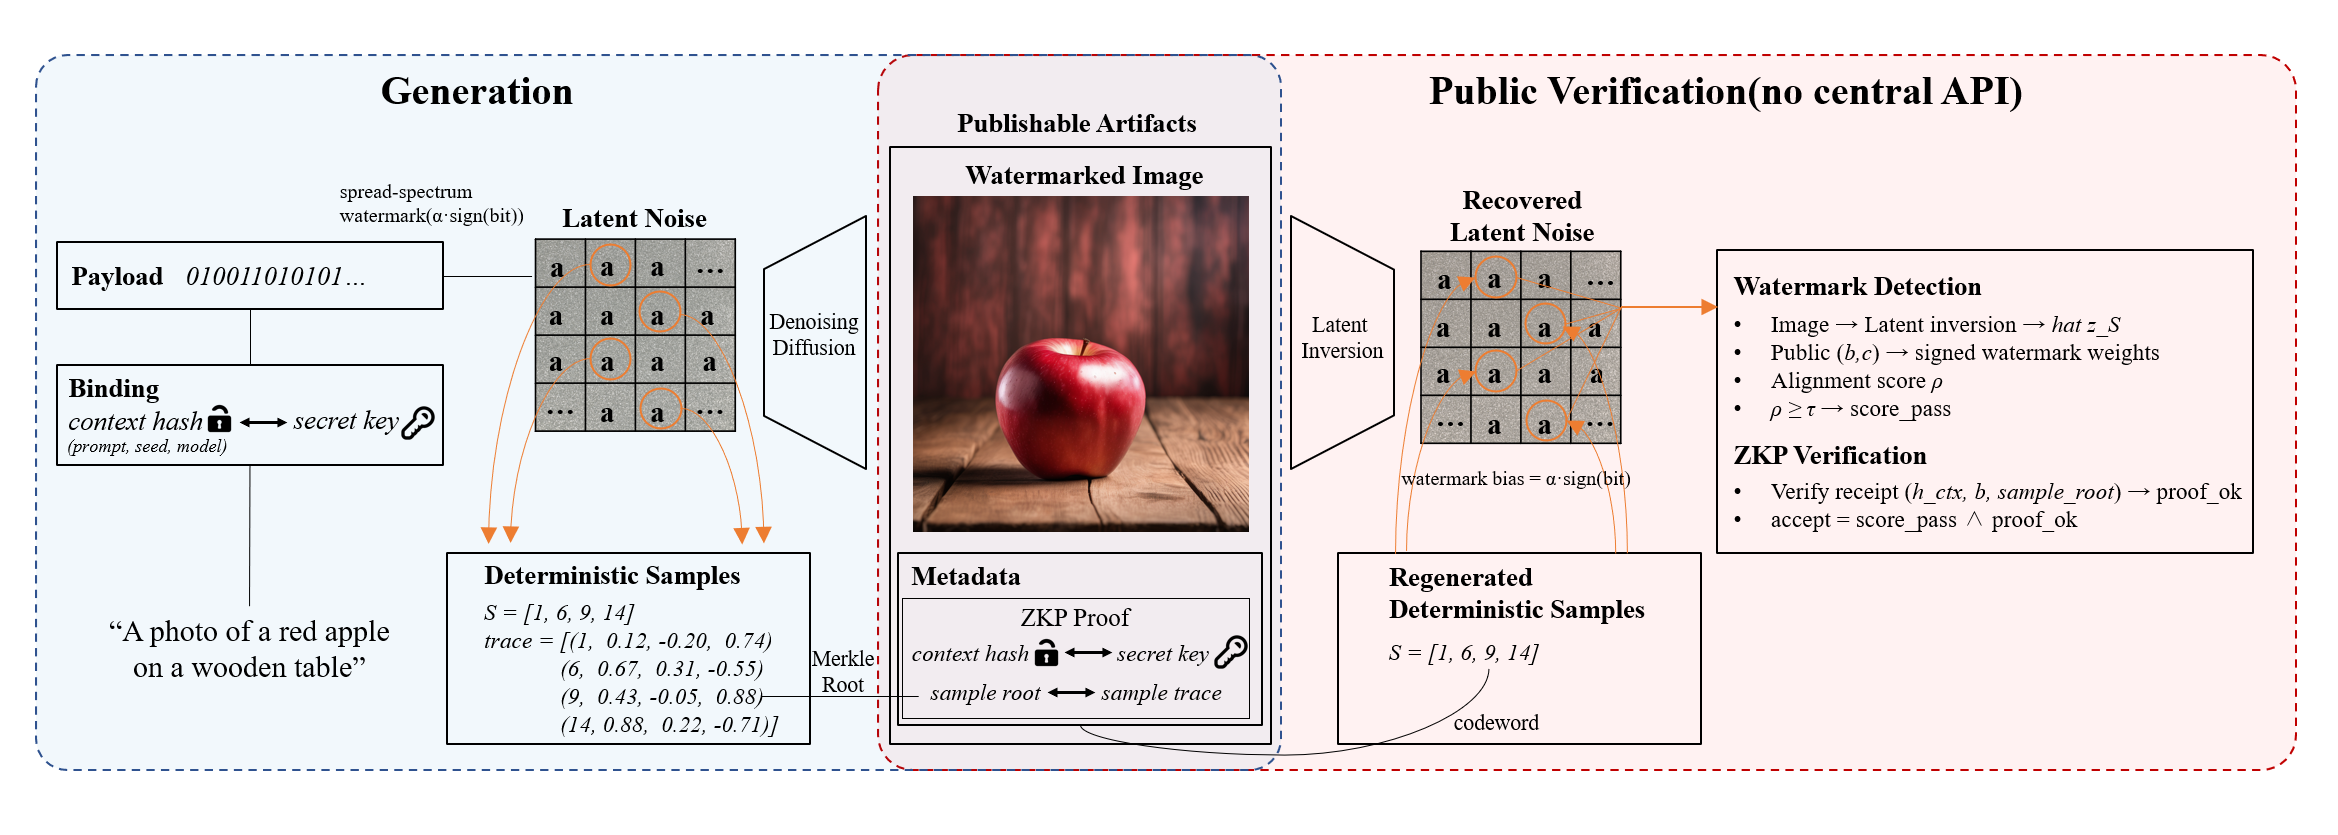
\includegraphics[width=\textwidth]{figures/ch04_source_ppmark_overview.png}
    \caption{PP-Mark generation and public verification workflow}
    \label{fig:ch4-overview}
\end{figure}

\subsection{Context-Bound Binding and Payload Construction}
\label{subsec:ch4-binding-payload}

Let $p$ be the prompt, $s$ the generation seed, \PPModelID{} the model
identifier, and $W\times H$ the output resolution.  Domain-separated hashing
first constructs a context hash and then mixes that public context with the secret
binding key:

\begin{equation}
\begin{aligned}
    h_p
        &= H(p),\\
    \PPContextHash
        &= H(\texttt{ctx\_hash}\parallel h_p\parallel\PPModelID\parallel
             s\parallel W\parallel H),\\
    \PPBinding
        &= H(\texttt{ctx\_hash}\parallel\PPContextHash\parallel\PPSecretKey).
\end{aligned}
\label{eq:ch4-binding-chain}
\end{equation}

Changing the prompt, seed, model identifier, or resolution changes
\PPContextHash{} and hence \PPBinding{}.  The prompt itself need not be placed in
the proof witness; its digest is sufficient for the binding relation.  Domain
separation prevents the same hash invocation from being interpreted as another
protocol field.

The public binding becomes a fixed-length watermark message and codeword:

\begin{equation}
    \PPPayload=\operatorname{Trunc}(\PPBinding),
    \qquad
    \PPCodeword=\operatorname{RS}(\PPPayload),
    \qquad
    \mathbf{r}=\operatorname{Bits}(\PPCodeword).
\label{eq:ch4-payload-codeword}
\end{equation}

Reed--Solomon expansion supplies a redundant binary sequence \(\mathbf r\) that
can be spread across the latent space.  This sequence is public once \PPBinding{}
is published, but the proof must still show that \PPBinding{} is consistent with a
valid secret-key witness.  Public reconstructability is necessary for independent
score computation; it is not permission to choose a new binding after inspecting
the target image.

The exact image enters after the trace has been committed.  Let
\(\mathsf{root}_{\mathrm{tr}}\) denote the Merkle root of the sampled trace and let
\PPImageHash{} be SHA-256 of deterministically canonicalized pixels.  The public
challenge material is

\begin{equation}
\begin{aligned}
    u
        &= (\PPImageHash,\PPContextHash,\mathsf{root}_{\mathrm{tr}}),\\
    \mathsf{seed}_{\mathrm{open}}
        &= H(\texttt{ppmark\_opening\_v1}\parallel u),\\
    \PPOpeningSet
        &= \operatorname{DeriveOpen}
           (\mathsf{seed}_{\mathrm{open}},\PPOpeningCount,\PPSampleCount).
\end{aligned}
\label{eq:ch4-opening-challenge}
\end{equation}

This ordering matters.  The root fixes the trace before the opening set is known,
and \PPImageHash{} prevents a receipt prepared for one exact image from being
replayed unchanged on another.  A cryptographic pixel hash is chosen instead of a
perceptual hash because a perceptual collision neighborhood would create an
explicit replay region.  The consequence is intentional but operationally
important: recompression, crop, resize, or any other pixel change invalidates the
receipt and requires proof re-issuance for the edited variant.

\subsection{Deterministic Sampling and Latent Watermark Embedding}
\label{subsec:ch4-sampling-embedding}

The codeword deterministically selects \PPSampleCount{} latent locations,

\begin{equation}
    \PPSampleSet
        =\operatorname{DeterministicSample}
          (\PPCodeword,\PPSampleCount),
    \qquad
    \operatorname{idx}(x,y)
        =H(\PPBinding\parallel x\parallel y\parallel777)\bmod L,
\label{eq:ch4-deterministic-sampling}
\end{equation}

where $L=|\mathbf r|$.  Any verifier given the same binding and public parameters
therefore reconstructs the same sample positions and coordinate-to-bit mapping.
The implementation uses one fixed reference latent channel.  Deterministic
spreading lets the detector aggregate a weak local signal over many positions and
keeps the sampled trace auditable.

For every latent index $i$, the binding also determines a pseudo-random Gaussian
baseline.  The construction maps a 32-bit hash-derived integer through a fixed
lookup table for the inverse normal CDF, $F^{-1}$:

\begin{equation}
\begin{aligned}
    u_i
        &=H(\PPBinding\parallel(i+1))\bmod2^{32},\\
    g_i
        &=F^{-1}\!\left(\frac{u_i}{2^{32}}\right),\\
    r_i
        &=2\,\mathbf r_{\operatorname{idx}(x,y)}-1,\\
    z_i
        &=g_i+\alpha r_i.
\end{aligned}
\label{eq:ch4-latent-embedding}
\end{equation}

Here $r_i\in\{-1,+1\}$ is the watermark sign and \(\alpha\) controls embedding
strength.  To preserve stable latent variance, the initialized latent and effective
strength are normalized as

\begin{equation}
    z_i^{(0)}=\frac{z_i}{\sqrt{1+\alpha^2}},
    \qquad
    \alpha_{\mathrm{eff}}
        =\frac{\alpha}{\sqrt{1+\alpha^2}}.
\label{eq:ch4-latent-normalization}
\end{equation}

For each $i\in\PPSampleSet$, the generator records the tuple
\((i,g_i,z_i^{(0)},\beta_i)\) in Q18 fixed-point form, where the committed bit
\(\beta_i=\mathbf r_{\operatorname{idx}(i)}\) for an honestly generated trace.
Those tuples constitute \PPTrace{}.  Fixed-point representation makes the proof
program's arithmetic deterministic; it also means that the verified relation is
the registered Q18 relation rather than an unspecified real-number computation.

The public verifier applies DDIM inversion to the candidate image $I$ and
obtains an estimate \(\widehat z^{(0)}\).  The expected watermark component at a
sampled position is $w_i=\alpha_{\mathrm{eff}}r_i$.  The normalized correlation
score is

\begin{equation}
    \PPDetectionScore
        =\frac{
            \left|
                \left\langle
                    \widehat z^{(0)}_{\PPSampleSet},
                    w_{\PPSampleSet}
                \right\rangle
            \right|
        }{
            \left\lVert w_{\PPSampleSet}\right\rVert_2
        }.
\label{eq:ch4-detection-score}
\end{equation}

The score interpretation depends on inversion error.  Write
\(\epsilon_i=\widehat z_i^{(0)}-z_i^{(0)}\).  The source analysis uses the
following empirical statistical condition.

\begin{assumption}[Inversion-residual condition]
\label{ass:ch4-inversion-residual}
The residuals \(\epsilon_i\) are approximately zero mean and have bounded moderate
correlation with the watermark signs $r_i$ over the registered sample positions.
\end{assumption}

Under Assumption~\ref{ass:ch4-inversion-residual}, the watermark term accumulates
coherently, while the Gaussian baseline and residual terms do not systematically
cancel it.  This is not asserted as an architecture-independent fact.  It is
checked empirically for Stable Diffusion 2.1 and SDXL in
Section~\ref{subsec:ch4-efficiency-generalization}.

\subsection{Trace Commitment and SP1 Proof Generation}
\label{subsec:ch4-trace-proof}

The sampled Q18 trace is committed with a Merkle tree.  A leaf hashes the sample
index, Gaussian baseline, normalized latent value, and payload bit; internal nodes
hash ordered child values until one root \(\mathsf{root}_{\mathrm{tr}}\) remains.
The root fixes the trace economically, while authentication paths let the proof
program check membership of opened tuples~\cite{merkle1988signature}.  The opening
digest commits the ordered tuples selected by \PPOpeningSet{}.

The SP1 receipt \PPReceipt{} attests that there exists a private witness

\begin{equation}
    \PPPrivateWitness
        =(
            \PPSecretKey,
            \PPCodeword,
            \PPTrace,
            \mathsf{paths}
          )
\label{eq:ch4-private-witness}
\end{equation}

consistent with the public statement

\begin{equation}
\begin{aligned}
    \PPPublicStatement
        =(&\PPBinding,
           \mathsf{root}_{\mathrm{tr}},
           \mathsf{digest}_{\mathrm{open}},
           \mathsf{seed}_{\mathrm{open}},
           \PPOpeningCount,
           \alpha_{\mathrm{eff}},
           \PPContextHash,\\
          &H(F^{-1}),
           \PPSampleCount,
           \PPImageHash).
\end{aligned}
\label{eq:ch4-public-statement}
\end{equation}

The image hash is shown explicitly in
Equation~\eqref{eq:ch4-public-statement} because it is an input to the opening
challenge even though image pixels are not a private circuit witness.  The lookup
table hash fixes the numerical inverse-CDF implementation, and the public sample
count makes the trace dimension auditable.

The proof program evaluates a composite predicate

\begin{equation}
    \mathcal P(\PPPublicStatement,\PPPrivateWitness)
        =P_1\land P_2\land P_3\land P_4,
\label{eq:ch4-composite-predicate}
\end{equation}

with the following obligations:

\begin{align}
P_1:
    &\quad
    \PPBinding
      =H(\texttt{ctx\_hash}\parallel\PPContextHash\parallel\PPSecretKey),
\label{eq:ch4-predicate-p1}\\
P_2:
    &\quad
    \operatorname{MerkleRoot}(\PPTrace)
      =\mathsf{root}_{\mathrm{tr}},
\label{eq:ch4-predicate-p2}\\
P_3:
    &\quad
    \begin{aligned}
    \PPOpeningSet
       &=\operatorname{DeriveOpen}
         (\mathsf{seed}_{\mathrm{open}},\PPOpeningCount,\PPSampleCount),\\
    \mathsf{digest}_{\mathrm{open}}
       &=H\!\left(
           \{\mathsf{leaf\_tuple}_i\}_{i\in\PPOpeningSet}
         \right),
    \end{aligned}
\label{eq:ch4-predicate-p3}\\
P_4:
    &\quad
    \forall i\in\PPOpeningSet:\;
    \begin{cases}
       \beta_i=\mathbf r_{\operatorname{idx}(i)},\\
       u_i=H(\PPBinding\parallel(i+1))\bmod2^{32},\\
       g_i=F^{-1}(u_i/2^{32}),\\
       z_i^{(0)}
          =g_i+\alpha_{\mathrm{eff}}
             \bigl(2\beta_i-1\bigr)
             \pmod{\mathrm{Q18}}.
    \end{cases}
\label{eq:ch4-predicate-p4}
\end{align}

$P_1$ binds the public value to possession of the secret-key witness.  $P_2$
fixes the sampled trace under the published root.  $P_3$ binds the opened tuples
to the image-derived challenge.  $P_4$ checks that every opened tuple follows
the binding-derived payload, Gaussian lookup, and registered embedding equation.
The last obligation is essential: merely checking that a committed tuple satisfies
an arithmetic relation chosen by the prover would permit tautological witnesses.

The circuit's negative boundary is as important as its checked obligations.  It
does not execute the text encoder, denoising trajectory, decoder, canonicalization
outside the registered hash input, or full DDIM inversion inside SP1.  Image-side
signal presence is evaluated by Equation~\eqref{eq:ch4-detection-score}; the proof
side checks consistency of the opened committed relation.  Full acceptance joins
these two independently visible conditions.

\subsection{Public Verification Modes and Formal Security Guarantee}
\label{subsec:ch4-verification-security}

PP-Mark exposes two modes rather than one ambiguous ``verified'' label.

\paragraph{PP-Mark(score).}
The verifier reconstructs the binding-derived sign pattern, DDIM-inverts the
image, computes \PPDetectionScore{}, and reports whether
\(\PPDetectionScore\geq\PPThreshold\).  The threshold is calibrated on clean
images for a target false-positive rate.  This mode is fast and can tolerate
moderate lossy transformations through soft correlation and alignment search.  It
is only statistical screening.  It does not establish that a secret-key holder
committed a trace or that the image is accompanied by a valid receipt.

\paragraph{Full acceptance.}
The verifier additionally canonicalizes the pixels, computes \PPImageHash{},
reconstructs the image-bound opening challenge, and verifies \PPReceipt{} against
\PPPublicStatement{}.  It returns a positive decision only when both the score and
receipt checks pass, as in Equation~\eqref{eq:ch4-intro-accept}.  This mode is
appropriate when the exact published object and a portable verification artifact
are available.  Its meaning is ``verified relative to the declared binding,'' not
``factually true'' or ``human-authored.''

Table~\ref{tab:ch4-threat-coverage} records the different surfaces covered by the
two modes.  A score can screen an external attack under the calibrated detector,
but a malicious generator that never embedded the registered signal can choose
metadata adversarially.  The proof-bearing mode adds a check on the binding and
committed trace without disclosing \PPSecretKey{}.

\begin{table}[H]
    \centering
    \caption{Threat coverage by verification mode}
    \label{tab:ch4-threat-coverage}
    \small
    \setlength{\tabcolsep}{7pt}
    \renewcommand{\arraystretch}{1.15}
    \begin{tabular}{@{}p{0.58\textwidth}cc@{}}
        \toprule
        Threat condition & Score & Accept \\
        \midrule
        External adversary without \PPSecretKey{} & \(\checkmark\) & \(\checkmark\) \\
        Generator fraud without registered embedding & \(\times\) & \(\checkmark\) \\
        Third-party audit without key disclosure & \(\times\) & \(\checkmark\) \\
        \bottomrule
    \end{tabular}
\end{table}

The formal statement makes the remaining failure probability visible.  Let
\PPLegitimateSet{} be the set of image--receipt pairs produced by the registered
generator, and suppose a committed trace contains at least \PPBadPositions{}
positions that violate the honest embedding relation.

\begin{assumption}[Cryptographic verification condition]
\label{ass:ch4-cryptographic}
SHA-256 is collision resistant and is modeled as a random oracle for derivation of
the post-commitment opening challenge~\cite{bellare1993randomoracle}; SP1 is computationally sound for security
parameter \(\lambda\); and the adversary does not possess \PPSecretKey{}.
\end{assumption}

\begin{theorem}[Unforgeability with partial opening]
\label{thm:ch4-unforgeability}
Under Assumption~\ref{ass:ch4-cryptographic}, for every probabilistic
polynomial-time adversary \(\mathcal A\) that commits a trace with at least
\PPBadPositions{} violating positions,
\begin{equation}
\begin{aligned}
&\Pr\!\left[
  \mathsf{PPMark}_{\mathrm{accept}}(I^*,\mathrm{md}^*,\PPReceipt^*)=1
  \;\land\;
  (I^*,\PPReceipt^*)\notin\PPLegitimateSet
\right]\\
&\quad\leq
  \operatorname{Adv}^{\mathrm{cr}}_{H}(\mathcal A)
  +\operatorname{Adv}^{\mathrm{sound}}_{\mathrm{SP1}}(\mathcal A)
  +\frac{
      \binom{\PPSampleCount-\PPBadPositions}{\PPOpeningCount}
    }{
      \binom{\PPSampleCount}{\PPOpeningCount}
    }\\
&\quad\leq
  \operatorname{Adv}^{\mathrm{cr}}_{H}(\mathcal A)
  +\operatorname{Adv}^{\mathrm{sound}}_{\mathrm{SP1}}(\mathcal A)
  +\left(1-\frac{\PPBadPositions}{\PPSampleCount}\right)^{\PPOpeningCount}.
\end{aligned}
\label{eq:ch4-unforgeability-bound}
\end{equation}
\end{theorem}

\begin{proof}[Proof sketch]
A verifying forged receipt has three relevant routes.  Reusing a public binding
with a different secret witness violates the hash-binding relation, and altering a
trace while preserving its root violates Merkle collision resistance.  Otherwise,
SP1 soundness implies that the composite predicate has a satisfying witness except
with its stated advantage.  Conditional on fixed commitments, the image-bound
challenge selects a uniformly modeled \PPOpeningCount-subset of the
\PPSampleCount{} positions.  The receipt can avoid detection of all
\PPBadPositions{} inconsistent positions only when the opening contains none of
them.  The exact hypergeometric probability of that event is the binomial ratio in
Equation~\eqref{eq:ch4-unforgeability-bound}, which is at most
\((1-\PPBadPositions/\PPSampleCount)^{\PPOpeningCount}\).  The union bound over
hash, proof-soundness, and missed-opening events yields the result.  Requiring the
score can only further restrict acceptance; it does not enlarge this upper bound.
\end{proof}

For the implemented \(\PPSampleCount=1000\) and
\(\PPOpeningCount=32\), the partial-opening term is approximately
\(2^{-6.3}\) when \(\PPBadPositions=0.125\PPSampleCount\), corresponding to a
98.7\% chance that the opening intersects the cheating set.  When half of the
trace positions violate the relation, the term is \(2^{-32}\).  Small cheating
sets are less likely to be opened, which is why the calibrated score remains a
separate condition.  This is a two-layer defense under explicit assumptions, not
a claim that either layer detects every possible deviation.

The theorem also does not repair key compromise.  If \PPSecretKey{} is disclosed,
an adversary can construct bindings and witnesses under that key.  Rotation,
epoch identifiers, public revocation information, and secure key storage are
therefore deployment obligations.  Similarly, if a proof artifact is detached or
corrupted, the image returns to an unverified state rather than falling back to a
stronger claim based on its score.

\section{Experimental Evaluation}
\label{sec:ch4-evaluation}

\subsection{Experimental Setup and Calibration}
\label{subsec:ch4-experimental-setup}

The primary experiments use Stable Diffusion 2.1 base with a DDIM scheduler, 50
inference steps, and classifier-free guidance scale 7.5.  Prompts are drawn from
the Stable-Diffusion-Prompts collection.  Unless an ablation states otherwise,
PP-Mark uses embedding strength \(\alpha=4.0\),
\(\PPSampleCount=1000\), and \(\PPOpeningCount=32\).  Generation, embedding,
inversion, and detector measurements run on an NVIDIA H100 PCIe 80 GB GPU; SP1
measurements use the same server with an Intel Xeon Gold 6542Y processor.

Each detector threshold targets a 1\% false-positive rate (FPR) on clean images
generated under the matching model settings.  The main forgery metric is forgery
acceptance rate (FAR) at that threshold.  Removal and transformation experiments
report true-positive rate (TPR) after the attack.  A score-mode result concerns
only the calibrated detector criterion.  Full acceptance additionally requires a
valid receipt.  Keeping those denominators distinct prevents a robust score from
being misreported as cryptographic acceptance.

The first experiment isolates the acceptance architecture before comparing
watermark methods.  Four interfaces are evaluated on 100 images under two targeted
attacks.  `Sig-only' accepts correctly signed metadata.  `Sig+Score' requires a
signature and a positive detector score.  PP-Mark(score) fixes the binding through
the secret-key construction but performs only statistical screening.
PP-Mark(accept) adds the SP1 receipt.

In the fabricated-binding attack, an adversary controlling only the comparison
metadata-signing key tests 10,000 random candidate bindings per image and retains
the one with the highest score.  The mean best score is 3.88, above the calibrated
\(\PPThreshold=2.47\).  In the compliance-bypass attack, the adversary signs
plausible metadata for a clean image without embedding the registered signal.
Table~\ref{tab:ch4-verification-ablation} reproduces the source outcomes.

\begin{table}[H]
    \centering
    \caption{Forgery acceptance by verification architecture}
    \label{tab:ch4-verification-ablation}
    \small
    \setlength{\tabcolsep}{4.2pt}
    \renewcommand{\arraystretch}{1.15}
    \begin{tabular}{@{}lcccc@{}}
        \toprule
        Attack
            & Sig-only
            & Sig+Score
            & \begin{tabular}[c]{@{}c@{}}PP-Mark\\(score)\end{tabular}
            & \begin{tabular}[c]{@{}c@{}}PP-Mark\\(accept)\end{tabular} \\
        \midrule
        Fabricated binding
            & 1.00 & 1.00 & \(\leq0.01^{\dagger}\) & 0.00 \\
        Compliance bypass
            & 1.00 & 0.00 & \(\leq0.01^{\dagger}\) & 0.00 \\
        \bottomrule
    \end{tabular}

    \vspace{2pt}
    \parbox{0.94\textwidth}{\footnotesize
    FAR at a 1\% clean-calibrated FPR; \(n=100\) per attack.
    \(^{\dagger}\)The bound is the calibrated FPR; 0 of 100 trials were
    observed positive.}
\end{table}

Signature-only verification accepts both attacks because it authenticates metadata
controlled by the adversary, not the embedding relation.  Adding a score blocks a
clean submission but does not block search over bindings: all 100 instances find a
score-positive candidate.  The secret-key-derived PP-Mark binding removes that
search freedom, and neither 100-image set produces an observed score positive.
Full acceptance also checks the receipt and records zero observed acceptances.
These finite results support the conjunctive interface; they do not replace the
conditional bound in Theorem~\ref{thm:ch4-unforgeability}.

A post-submission signature control further separates exact integrity from
embedding compliance.  Bare-Sig uses Ed25519 over the canonical pixel hash;
Context-Sig additionally signs the context hash and \(\PPBinding\).  Both are
appropriate exact-image integrity controls under a trusted signer, but neither
proves that the signer actually embedded a watermark.  Table~\ref{tab:ch4-signature-control}
reports the fixed 100-image comparison.

\begin{table}[tbp]
    \centering
    \caption{Exact-signature and embedding-compliance controls}
    \label{tab:ch4-signature-control}
    \footnotesize
    \setlength{\tabcolsep}{3pt}
    \renewcommand{\arraystretch}{1.12}
    \begin{tabular}{@{}
        >{\raggedright\arraybackslash}p{0.32\textwidth}
        >{\centering\arraybackslash}p{0.17\textwidth}
        >{\centering\arraybackslash}p{0.18\textwidth}
        >{\centering\arraybackslash}p{0.23\textwidth}@{}}
        \toprule
        \textbf{Test (\(n=100\))} & \textbf{Bare-Sig} &
        \textbf{Context-Sig} & \textbf{PP-Mark evidence} \\
        \midrule
        Original verifies & 100/100 & 100/100 & -- \\
        Cross-image replay accepted & 0/100 & 0/100 & -- \\
        Context substitution accepted & 100/100 & 0/100 & -- \\
        Authorized signer signs an unwatermarked image &
        100/100 & 100/100 & 0/100 score or accept \\
        JPEG quality 25 after signing & 0/100 valid & 0/100 valid &
        94/100 score detections \\
        75\% crop--resize after signing & 0/100 valid & 0/100 valid &
        87/100 score detections \\
        \bottomrule
    \end{tabular}
\end{table}

For exact integrity alone, a conventional signature is simpler and preferable.
PP-Mark's additional contribution is different: the receipt and score jointly
test an embedding relation, while the image-side signal remains detectable after
selected transformations that invalidate exact signatures.  The comparison does
not claim that a large proof should replace a signature when no embedding-
compliance statement is required.

\subsection{Forgery Attacks}
\label{subsec:ch4-forgery-attacks}

\paragraph{Black-box imprint transfer.}
The black-box evaluation tests whether an imprint extracted from one watermarked
reference can be transferred to an arbitrary cover image and attributed to the
reference source~\cite{muller2025blackbox}.  A fixed pool contains 200 prompts,
split equally between calibration and evaluation, and 100 fixed cover--reference
pairs are reused for every method.  Stable Diffusion 2.1 serves as both the target
and proxy architecture.  Optimization budgets of 50, 100, and 150 steps are
evaluated.

Before cross-method transfer, a direct sanity check attacks Tree-Ring and Gaussian
Shading with their own imprints.  Tree-Ring reaches FARs from 0.92 to 0.97 across
the three step budgets, and Gaussian Shading reaches 1.00 throughout.  The
pipeline therefore produces the targeted attribution effect before it is applied
to other detectors.

Table~\ref{tab:ch4-blackbox-transfer} aggregates the three step budgets for
Tree-Ring-sourced and Gaussian-Shading-sourced imprints.  The source table also
reports percentage changes against PP-Mark(score), but those ratios use only one
and two PP-Mark positive trials, respectively.  Absolute FAR, confidence
intervals, and one-sided Fisher tests are retained as the primary evidence.

\begin{table}[H]
    \centering
    \caption{Cross-method black-box imprint transfer}
    \label{tab:ch4-blackbox-transfer}
    \scriptsize
    \setlength{\tabcolsep}{5.2pt}
    \renewcommand{\arraystretch}{1.12}
    \begin{tabular}{@{}lcccc@{}}
        \toprule
        Method & FAR & 95\% CI & Relative \(\Delta\) (\%) & Fisher \(p\) \\
        \midrule
        \multicolumn{5}{@{}l}{\textit{Tree-Ring-sourced imprint}} \\
        TrustMark       & 0.0367 & 0.0184--0.0647 & +1000.0 & 0.0029 \\
        InvisMark       & 0.0300 & 0.0133--0.0500 &  +800.0 & 0.0102 \\
        RingID          & 0.0400 & 0.0208--0.0688 & +1100.0 & 0.0016 \\
        StableSig       & 0.0333 & 0.0161--0.0604 &  +900.0 & 0.0055 \\
        HiDDeN          & 0.0233 & 0.0094--0.0475 &  +600.0 & 0.0343 \\
        WIND            & 0.0100 & 0.0021--0.0289 &  +200.0 & 0.3119 \\
        PP-Mark(score)  & 0.0033 & 0.0001--0.0184 &       -- &     -- \\
        PP-Mark(accept) & 0.0000 & --              &       -- &     -- \\
        \midrule
        \multicolumn{5}{@{}l}{\textit{Gaussian-Shading-sourced imprint}} \\
        TrustMark       & 0.0267 & 0.0116--0.0519 & +300.0 & 0.0532 \\
        InvisMark       & 0.0167 & 0.0033--0.0333 & +150.0 & 0.2252 \\
        RingID          & 0.0133 & 0.0036--0.0338 & +100.0 & 0.3430 \\
        StableSig       & 0.0167 & 0.0054--0.0385 & +150.0 & 0.2252 \\
        HiDDeN          & 0.0233 & 0.0094--0.0475 & +250.0 & 0.0882 \\
        WIND            & 0.0100 & 0.0021--0.0289 &  +50.0 & 0.5000 \\
        PP-Mark(score)  & 0.0067 & 0.0008--0.0239 &      -- &     -- \\
        PP-Mark(accept) & 0.0000 & --              &      -- &     -- \\
        \bottomrule
    \end{tabular}

    \vspace{2pt}
    \parbox{0.95\textwidth}{\footnotesize
    FAR at 1\% FPR, aggregated across 50, 100, and 150 optimization steps.
    Relative \(\Delta\) is descriptive because its PP-Mark(score) denominators are
    one positive Tree-Ring-sourced trial and two positive Gaussian-Shading-sourced
    trials.}
\end{table}

PP-Mark(score) remains at or below the 1\% calibration floor: 0.0033 for the
Tree-Ring source and 0.0067 for the Gaussian-Shading source.  PP-Mark(accept)
records no accepted forgeries.  Tree-Ring-sourced differences for RingID, Stable
Signature, and HiDDeN are significant at 0.05 in the reported Fisher tests;
Gaussian-Shading-sourced comparisons do not reach that level.  The latter result
is not converted into a claim of method equality.  The absolute ordering and
intervals show low PP-Mark transfer in this fixed experiment, while the full mode
additionally refuses a receipt-free attribution.

\paragraph{White-box optimization.}
The white-box attacker receives each detector and its gradients and applies 150
projected-gradient steps under an \(\ell_\infty\) budget of
\(2/255\).  A score-mode forgery succeeds when the method's calibrated detector
crosses its threshold.  Average step counts and peak signal-to-noise ratio (PSNR)
are computed only among successful forgeries.  Table~\ref{tab:ch4-whitebox}
reports the Stable Diffusion 2.1 outcomes.

\begin{table}[H]
    \centering
    \caption{White-box forgery outcomes on Stable Diffusion 2.1}
    \label{tab:ch4-whitebox}
    \small
    \setlength{\tabcolsep}{8pt}
    \renewcommand{\arraystretch}{1.13}
    \begin{tabular}{@{}lccc@{}}
        \toprule
        Method & FAR at 1\% FPR & Avg. steps to FAR & Avg. PSNR \\
        \midrule
        TrustMark       & 1.00 &  2.41 & 75.73 \\
        InvisMark       & 1.00 &  3.07 & 72.67 \\
        StableSig       & 1.00 &  5.40 & 65.91 \\
        HiDDeN          & 1.00 &  8.08 & 62.96 \\
        RingID          & 1.00 &  2.26 & 74.51 \\
        WIND            & 1.00 & 22.20 & 55.76 \\
        PP-Mark(score)  & 0.76 & 17.42 & 67.69 \\
        PP-Mark(accept) & 0.00 &    -- &    -- \\
        \bottomrule
    \end{tabular}
\end{table}

Every comparison detector reaches a 1.00 FAR in this white-box setting.
PP-Mark(score) is also vulnerable to direct optimization, reaching 0.76 FAR.  This
result is precisely why a score-positive image is not labeled as publicly verified
provenance.  Pixel optimization changes \PPImageHash{}, hence the opening seed,
opened positions, and opening digest.  The attacker does not produce a matching
receipt, so PP-Mark(accept) records zero full acceptances.  The observed zero is
conditional on the tested budget and sample and is interpreted together with the
cryptographic assumptions, not as an attack-independent empirical probability.

\subsection{Removal and Transformation Attacks}
\label{subsec:ch4-removal-transform}

Forgery resistance is not sufficient if ordinary manipulation always destroys the
screening signal.  The next experiments therefore evaluate score-mode retention
under regeneration, multi-image steganalysis, gradient-free removal, and common
pixel or geometric transformations.  These tests do not claim that an old exact
receipt remains valid after editing; by design, any changed canonical pixel string
requires a new receipt.

\paragraph{Regeneration.}
Diffusion regeneration adds noise to a watermarked image and synthesizes it again,
a process known to remove some invisible pixel watermarks~\cite{zhao2024removable}.
Table~\ref{tab:ch4-regeneration} reports detector TPR at three source noise-step
settings.  PP-Mark retains 0.98 in all three, while several post-hoc methods fall
below 0.10.  Tree-Ring also remains high at 0.93--0.95, consistent with the
relative durability of signals embedded in the generation latent.

\begin{table}[H]
    \centering
    \caption{Detection after diffusion regeneration}
    \label{tab:ch4-regeneration}
    \small
    \setlength{\tabcolsep}{8pt}
    \renewcommand{\arraystretch}{1.13}
    \begin{tabular}{@{}lccc@{}}
        \toprule
        Method & 30 steps & 60 steps & 100 steps \\
        \midrule
        StableSig  & 0.04 & 0.02 & 0.03 \\
        HiDDeN     & 0.10 & 0.06 & 0.04 \\
        TrustMark  & 0.85 & 0.63 & 0.39 \\
        InvisMark  & 0.01 & 0.05 & 0.02 \\
        Tree-Ring  & 0.95 & 0.93 & 0.93 \\
        PP-Mark    & 0.98 & 0.98 & 0.98 \\
        \bottomrule
    \end{tabular}

    \vspace{2pt}
    \parbox{0.92\textwidth}{\footnotesize
    Values are score-mode TPR at the 1\% clean-calibrated FPR.}
\end{table}

\paragraph{Steganalysis.}
The multi-image attack averages residuals from $K$ watermarked reference
images, treats the average as a shared watermark estimate, and subtracts it from a
target.  Table~\ref{tab:ch4-steganalysis} shows that Stable Signature and Tree-Ring
lose much of their detection rate as more references are averaged.  TrustMark,
InvisMark, WIND, and PP-Mark remain highly detectable at larger $K$, consistent
with image-conditioned patterns that do not converge to one reusable residual.

\begin{table}[H]
    \centering
    \caption{Detection after multi-image steganalysis}
    \label{tab:ch4-steganalysis}
    \small
    \setlength{\tabcolsep}{11.5pt}
    \renewcommand{\arraystretch}{1.13}
    \begin{tabular}{@{}lcccc@{}}
        \toprule
        Method & \(K=10\) & \(K=100\) & \(K=500\) & \(K=1000\) \\
        \midrule
        StableSig & 0.200 & 0.200 & 0.173 & 0.171 \\
        Tree-Ring & 0.190 & 0.020 & 0.038 & 0.035 \\
        TrustMark & 0.990 & 0.960 & 0.960 & 0.960 \\
        InvisMark & 1.000 & 1.000 & 1.000 & 1.000 \\
        WIND      & 1.000 & 1.000 & 1.000 & 1.000 \\
        PP-Mark   & 0.864 & 0.959 & 0.963 & 0.958 \\
        \bottomrule
    \end{tabular}

    \vspace{2pt}
    \parbox{0.92\textwidth}{\footnotesize
    Values are score-mode TPR at the 1\% clean-calibrated FPR.}
\end{table}

\paragraph{Gradient-free SPSA.}
Simultaneous perturbation stochastic approximation (SPSA) estimates a search
direction with score queries rather than detector gradients~\cite{spall1992spsa}.
For removal, the adversary minimizes the PP-Mark score for 50 steps.  As shown in
Figure~\ref{fig:ch4-spsa-removal}, the score can cross below
\PPThreshold{}, but only after image quality collapses: successful low-score
points have PSNR from 4.7 to 6.9, and no removal satisfies the source validity
criterion of PSNR at least 30.  This result is evidence under one attack and
quality constraint, not a general impossibility of black-box removal.

\begin{figure}[H]
    \centering
    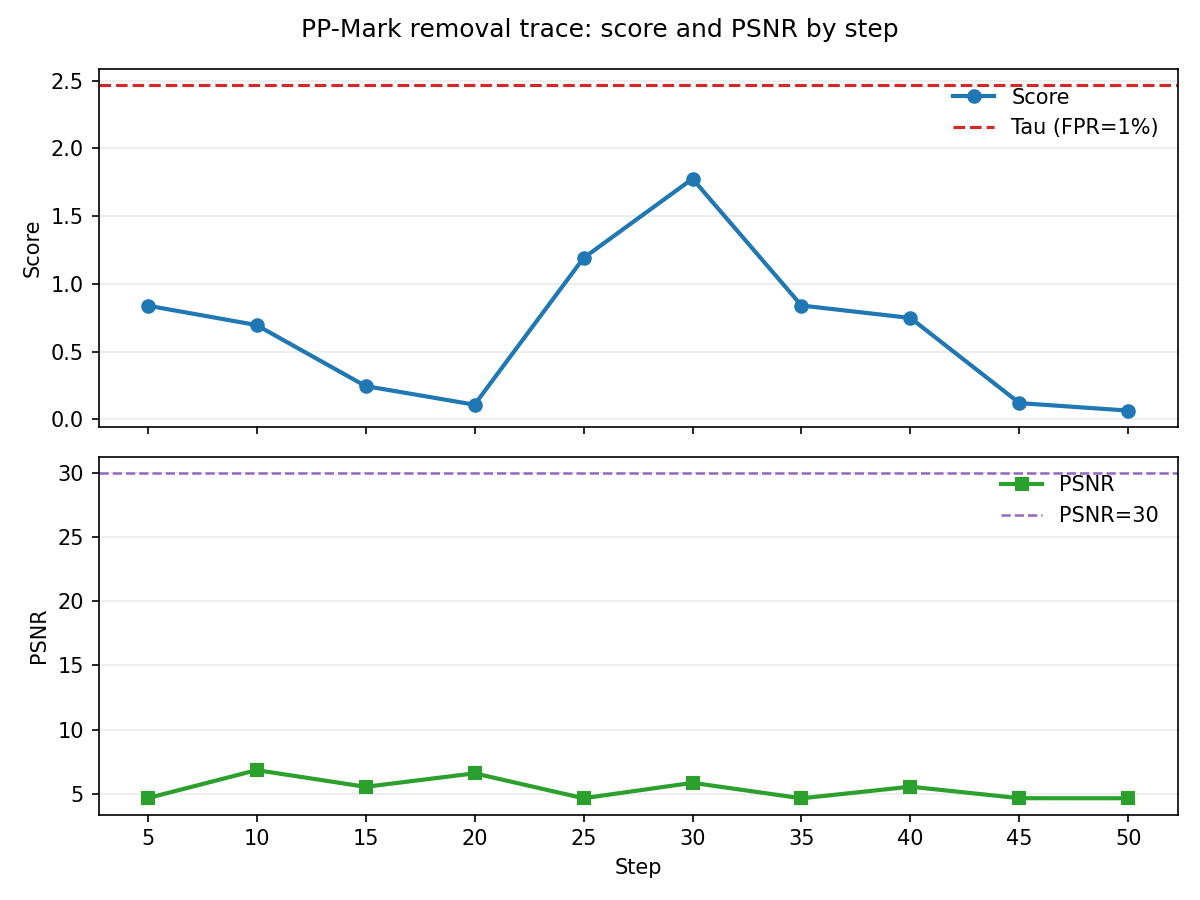
\includegraphics[width=0.82\textwidth]{figures/ch04_source_spsa_removal.png}
    \caption{SPSA removal trajectory}
    \label{fig:ch4-spsa-removal}
\end{figure}

In the complementary SPSA forgery test, score-mode FARs at 50, 100, and 150 steps
are 0.02, 0.00, and 0.01, with corresponding mean PSNRs 6.55, 6.61, and 6.63.
The aggregate FAR is 0.01 at mean PSNR 6.60.  The low-quality solutions again
show that reporting attack success without a perceptual constraint would be
misleading.  Full acceptance would additionally require a receipt for the changed
image.

\paragraph{Pixel and geometric transformations.}
The detector uses an alignment search for geometric synchronization.  Table
~\ref{tab:ch4-transformations} reports score-mode TPR for Stable Diffusion 2.1 and
SDXL.  Compression, blur, additive noise, and brightness changes retain TPRs from
0.86 to 1.00.  Random crop with resize is the weakest SDXL case at 0.74, while a
75-degree rotation reaches 0.85 on SD 2.1 and 0.97 on SDXL after synchronization.

\begin{table}[H]
    \centering
    \caption{Detection after pixel and geometric transformations}
    \label{tab:ch4-transformations}
    \small
    \setlength{\tabcolsep}{12pt}
    \renewcommand{\arraystretch}{1.15}
    \begin{tabular}{@{}lcc@{}}
        \toprule
        Transformation & SD 2.1 TPR & SDXL TPR \\
        \midrule
        JPEG, quality 25            & 0.94 & 1.00 \\
        Blur, \(8\times8\)          & 1.00 & 1.00 \\
        Gaussian noise, \(\sigma=0.1\) & 0.86 & 0.95 \\
        Brightness, \(\times0.6\)   & 0.98 & 1.00 \\
        Random crop and resize, 75\% & 0.87 & 0.74 \\
        Rotation, \(75^{\circ}\)    & 0.85 & 0.97 \\
        \bottomrule
    \end{tabular}

    \vspace{2pt}
    \parbox{0.92\textwidth}{\footnotesize
    Score-mode TPR at the matching 1\% FPR; SDXL crop-and-resize uses \(n=50\).}
\end{table}

These transformation results define the role of PP-Mark(score), not the validity
of an old proof.  The canonical SHA-256 image hash changes under every listed
operation.  A transformed image may still be discovered by the statistical
screen, but it becomes PP-Mark-accepted only after a producer issues a receipt for
that exact transformed pixel representation.

A post-submission sequential test applies 75\% crop, bicubic resize, and JPEG
quality 25 to the same 100 SD 2.1 watermarked images with no survivor filtering.
Persistent success requires detection at every checkpoint; 80 of 100 images remain
detectable through the complete pipeline, compared with 87 of 100 after crop--
resize alone and 94 of 100 after JPEG alone.  The 80\% result measures cumulative
score degradation under one fixed three-operation pipeline.  It does not change
the exact-image boundary of PP-Mark(accept).

\subsection{Efficiency, Image Quality, and Model Generalization}
\label{subsec:ch4-efficiency-generalization}

The sample count controls detector variance, proof work, and receipt size.  The two
source ablations appear in Figure~\ref{fig:ch4-sampling-tradeoff}.  Increasing the
count from 200 to 1000 reduces the empirical
score standard deviation from 0.1409 to 0.1301, a 7.7\% decrease; increasing it
from 1000 to 1500 supplies only a further 3.0\% decrease.  SP1 proving time grows
from 32.309 s at 200 samples to 48.572 s at 1000 and 60.272 s at 1500.  The
selected value of 1000 is therefore an empirical operating point rather than a
universal optimum.  Concentration with larger samples supplies the statistical
motivation, while the source analysis uses the registered empirical calibration
rather than claiming an asymptotic detector guarantee~\cite{hoeffding1963}.

\begin{figure}[H]
    \centering
    \begin{subfigure}[t]{0.48\textwidth}
        \centering
        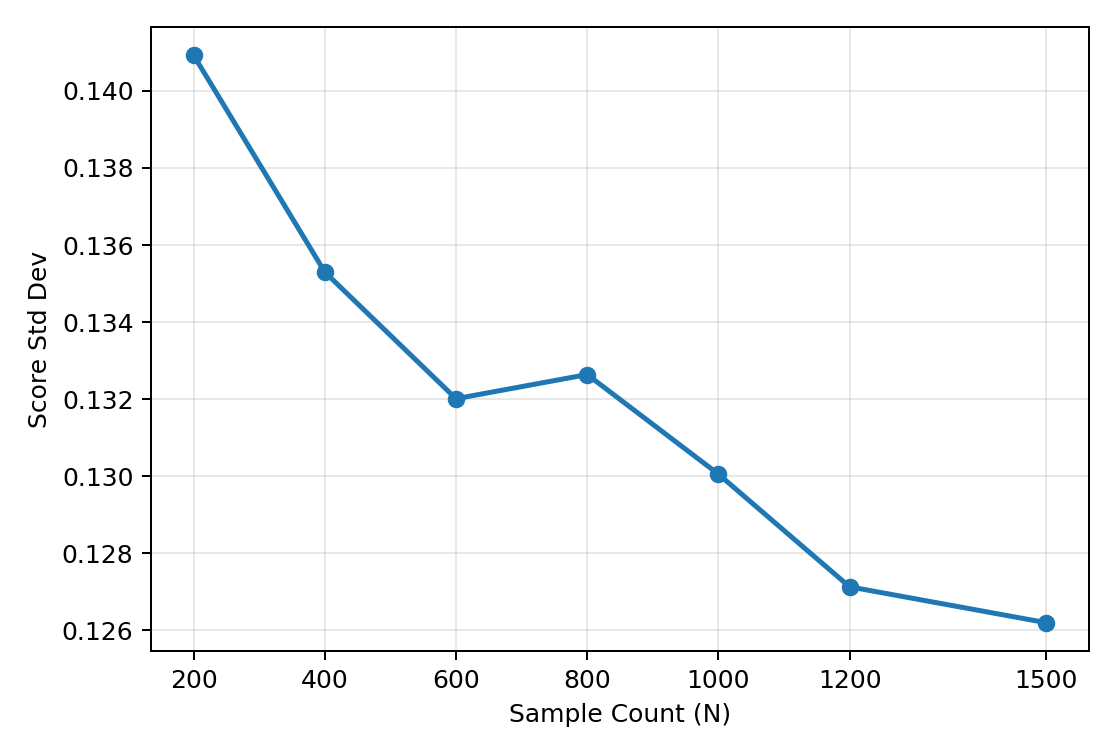
\includegraphics[width=\linewidth]{figures/ch04_source_sample_score_stability.png}
        \caption{Score variation}
        \label{fig:ch4-sample-score}
    \end{subfigure}
    \hfill
    \begin{subfigure}[t]{0.48\textwidth}
        \centering
        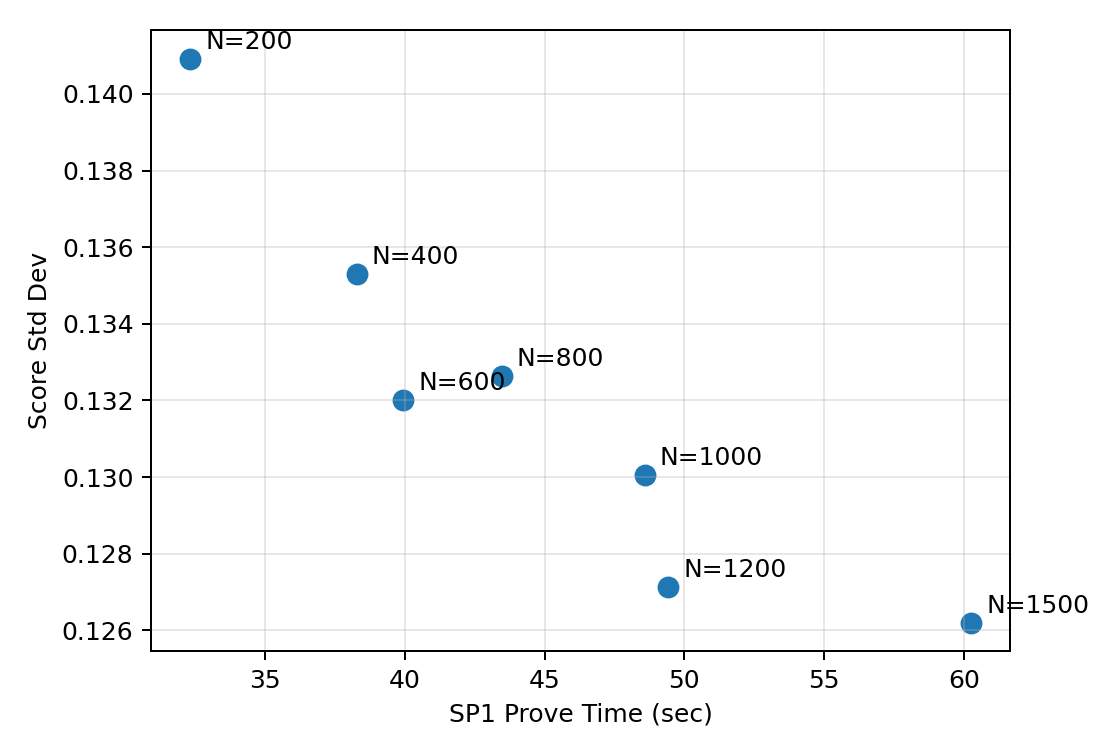
\includegraphics[width=\linewidth]{figures/ch04_source_score_proving_tradeoff.png}
        \caption{Proving time}
        \label{fig:ch4-score-proving}
    \end{subfigure}
    \caption{Sampling stability and SP1 proving trade-off}
    \label{fig:ch4-sampling-tradeoff}
\end{figure}

Table~\ref{tab:ch4-runtime} reports end-to-end runtimes on Stable Diffusion 2.1.
The score mode matches the Tree-Ring path at 0.89 s for embedding and 0.72 s for
verification.  Full acceptance adds 48.6 s for one-time proof generation and
7.59 s for receipt verification.  At
\(\PPSampleCount=1000\), the more precise SP1 checkpoints are 48.572 s proving
and 7.589 s verification, and the receipt occupies 40.68 MB.  The artifact is
therefore feasible for archival or on-request verification in the evaluated
environment, but it is costly for a per-upload streaming path.

\begin{table}[H]
    \centering
    \caption{End-to-end runtime on Stable Diffusion 2.1}
    \label{tab:ch4-runtime}
    \small
    \setlength{\tabcolsep}{15pt}
    \renewcommand{\arraystretch}{1.13}
    \begin{tabular}{@{}lcc@{}}
        \toprule
        Method & Embed or generate (s) & Verify (s) \\
        \midrule
        Tree-Ring        & 0.89 & 0.75 \\
        Gaussian Shading & 3.10 & 0.72 \\
        RingID           & 0.89 & 0.72 \\
        WIND             & 0.89 & 1.10 \\
        Stable Signature & 0.91 & 0.008 \\
        HiDDeN           & 0.001 & 0.001 \\
        TrustMark        & 0.013 & 0.004 \\
        InvisMark        & 0.002 & 0.009 \\
        PP-Mark(score)   & 0.89 & 0.72 \\
        PP-Mark(accept)  & \(0.89+48.6^{\dagger}\) & \(0.72+7.59^{\dagger}\) \\
        \bottomrule
    \end{tabular}

    \vspace{2pt}
    \parbox{0.92\textwidth}{\footnotesize
    \(^{\dagger}\)Additional SP1 proving and receipt-verification time at
    \(\PPSampleCount=1000\).}
\end{table}

After the submitted-paper evaluation, an SP1 v6.3.1 port with Merkle-work
optimization was rerun at the same \(\PPSampleCount=1000\) configuration.  It
reduced measured proving time from 48.572 s to 17.0 s and the receipt artifact from
40.68 MB to 2.81 MB.  This is reported as a post-submission implementation update,
not silently substituted into Table~\ref{tab:ch4-runtime} or the submitted attack
comparisons.  The update improves the engineering point but leaves the assurance
predicate and the distinction between routine score screening and one-time exact-
image proof generation unchanged.

Receipt size scales from 12.24 MB at 300 sampled positions to 65.96 MB at 1500;
the private witness grows from 254.69 KB to 1493.57 KB over the same range, while
the public input remains approximately 0.66 KB.  A STARK-to-SNARK wrapper or proof
aggregation could reduce distributed proof size, but that optimization is not
implemented or counted as a current result.

Embedding strength is selected with a tail-sensitive perceptual diagnostic.
Figure~\ref{fig:ch4-brisque} plots the 95th percentile of BRISQUE against
\(\alpha\).  Values from 3.0 through 4.0 remain approximately 34.1--34.9, whereas
4.5 rises to about 40.5.  The implemented \(\alpha=4.0\) retains the stronger
detection setting before this observed tail-quality degradation.  The underlying
study also reports KID 0.0011014 on one 500-image, 20-split configuration; because
that is one moderate-size setup, it is treated as supporting distributional
evidence rather than a definitive perceptual guarantee.

Post-submission matched-pool measurements place this result beside the evaluated
baselines in Table~\ref{tab:ch4-matched-quality}.  Lower BRISQUE is preferred,
KID is interpreted toward zero, and higher CLIP alignment is preferred.  PP-Mark
does not have the best value in every column; the defensible conclusion is that its
quality is comparable to several latent- and pixel-watermark baselines while its
full mode adds a different embedding-compliance guarantee.

\begin{table}[tbp]
    \centering
    \caption{Post-submission matched image-quality comparison}
    \label{tab:ch4-matched-quality}
    \footnotesize
    \setlength{\tabcolsep}{6pt}
    \renewcommand{\arraystretch}{1.10}
    \begin{tabular}{@{}lccc@{}}
        \toprule
        Method & BRISQUE p95 \(\downarrow\) &
        KID \(\times10^3\) \((\rightarrow0)\) & CLIP \(\times100\) \(\uparrow\) \\
        \midrule
        PP-Mark          & 34.14  & $1.101\pm0.202$   & 31.64 \\
        Gaussian Shading & 27.35  & $0.621\pm1.096$   & 32.42 \\
        HiDDeN           & 105.86 & $7.239\pm1.474$   & 31.30 \\
        InvisMark        & 31.36  & $-0.900\pm0.895$  & 32.53 \\
        RingID           & 34.64  & $-0.989\pm0.701$  & 32.41 \\
        Stable Signature & 32.69  & $-0.814\pm0.878$  & 32.50 \\
        Tree-Ring        & 41.90  & $-0.090\pm0.922$  & 32.30 \\
        WIND             & 27.42  & $-0.386\pm0.879$  & 32.28 \\
        TrustMark        & 29.44  & $-0.174\pm1.001$  & 32.54 \\
        \bottomrule
    \end{tabular}

    \vspace{2pt}
    \parbox{0.94\textwidth}{\footnotesize
    KID is an unbiased finite-sample estimator and can be slightly negative; such
    values are sampling estimates near zero, not negative distances.}
\end{table}

\begin{figure}[H]
    \centering
    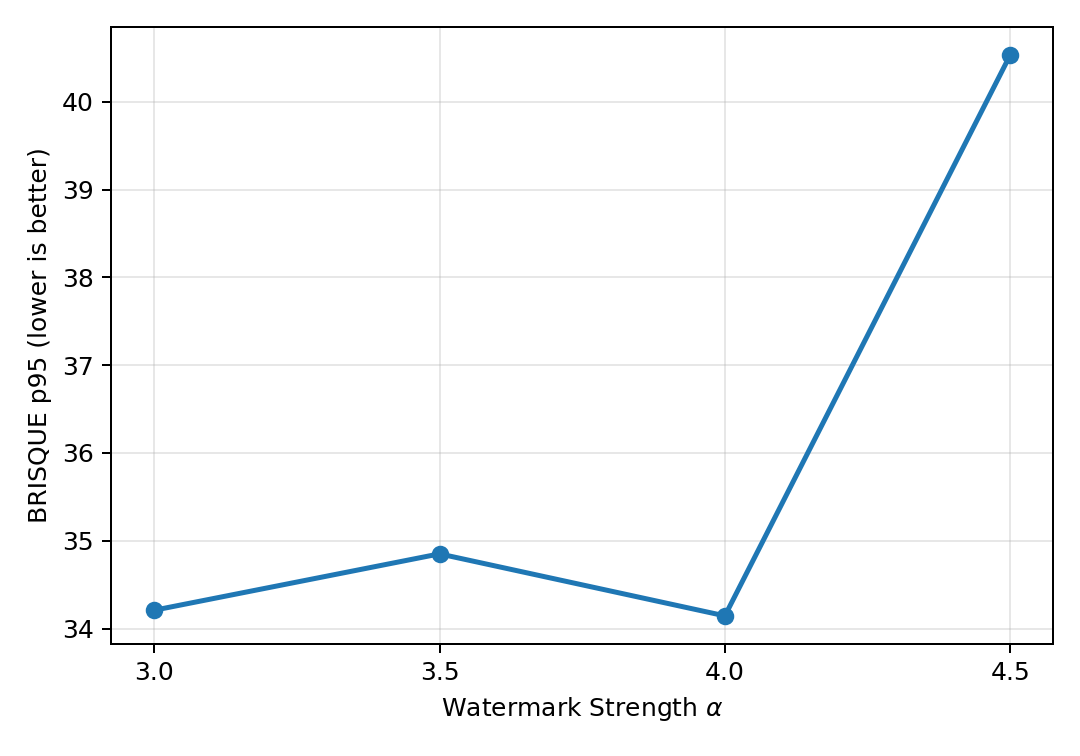
\includegraphics[width=0.78\textwidth]{figures/ch04_source_brisque_strength.png}
    \caption{Perceptual quality across embedding strengths}
    \label{fig:ch4-brisque}
\end{figure}

\paragraph{Inversion diagnostics.}
Assumption~\ref{ass:ch4-inversion-residual} is checked on 100 watermarked images
per latent-diffusion model.  On Stable Diffusion 2.1, the residual mean is
\(0.011\pm0.003\), the standard deviation is approximately 0.50, and the mean,
median, and maximum absolute residual--sign correlations are 0.30, 0.30, and
0.48.  The observed clean watermark score has mean 25.7 and minimum 17.4.  On
SDXL, the residual mean is \(-0.022\pm0.004\), with 95\% interval
\([-0.031,-0.013]\), standard deviation approximately 0.44, and mean, median, and
maximum absolute correlations 0.54, 0.55, and 0.66.  Correlation is stronger than
on SD 2.1, but it acts as shrinkage rather than complete cancellation in the
reported sample.

\paragraph{Bounded SDXL replication.}
The SDXL experiment uses 100 clean and 100 watermarked images per method, 50 DDIM
steps, \(\alpha=4.0\), and \(\PPSampleCount=1000\) on the 128-by-128 latent.
All thresholds are recalibrated to 1\% FPR on SDXL clean images.  PP-Mark's mean
watermarked score is 13.63 against \(\PPThreshold=2.47\), a 5.5-fold margin, and
all 100 clean watermarked evaluations cross the threshold.

Under Tree-Ring-sourced transfer, score-mode FARs at 50, 100, and 150 steps are
0.02, 0.00, and 0.01; under Gaussian-Shading-sourced transfer they are 0.01 at
every step.  The full mode records zero acceptances in all six conditions.  In the
SDXL white-box test, TrustMark and InvisMark each reach 1.00 FAR.  PP-Mark's score
mode reaches 0.11 with 95\% confidence interval 0.0562--0.1883, while the full
mode records 0.00.  These results show that the
registered construction can be run on two evaluated latent-diffusion models.
They do not establish architecture-agnostic generalization.

\paragraph{Limitations.}
Four limitations delimit the experimental conclusion.  First, proving time and
receipt size remain substantial at the selected sample count.  Second, the exact
image hash prevents unchanged receipt reuse after a benign edit; re-proving costs
about 48.6 s in the submitted environment and 17.0 s in the post-submission SP1
v6.3.1 update.  Third, the receipt must remain
attached or retrievable, and key rotation and revocation must operate correctly.
Fourth, geometric alignment remains imperfect for crop-and-resize on SDXL, and
only SD 2.1 and SDXL are tested.  The interface also does not account for
cumulative information exposed by repeated adaptive score queries.  That
dimension remains future work rather than a completed result in this chapter.

\section{Summary}
\label{sec:ch4-summary}

This chapter developed the \SecurePublicVerification{} axis of
\ClaimAlignedAssurance{}.  A hidden detector limits independent audit, whereas a
public detector exposes a score that can be queried or optimized.  PP-Mark
therefore keeps statistical screening separate from full acceptance, which
requires both image-side evidence and a publicly verifiable receipt.

The prompt hash, seed, model identifier, resolution, and producer-held key derive
a binding that determines the payload, sampled positions, Gaussian baselines, and
latent signs.  Q18 trace tuples are Merkle-committed, and the exact image hash
derives the post-commitment opening.  SP1 checks key binding, trace commitment,
the image-bound opening, and the opened embedding relation without disclosing the
secret key.

The two evidence layers remain experimentally distinct.  Search over 10,000
bindings defeats signature plus score, and white-box optimization raises the
public score on 76\% of the SD 2.1 covers, yet zero full acceptances are observed
in the reported forgery tests.  Score mode retains 0.74--1.00 TPR over the common
transformations and 0.98 after regeneration.  The exact-image proof is not
transform robust; an edited variant requires a new receipt.

The assurance statement remains conditional on hash resistance, SP1 soundness,
key control, the composite predicate, inversion behavior, and partial opening.
The circuit does not prove complete diffusion execution, semantic truth,
authorship, or legal identity.  Proof cost and persistence, key lifecycle,
geometric synchronization, two-model coverage, and adaptive queries remain
open limits.

Within those boundaries, PP-Mark demonstrates the chapter's central principle: a
public provenance claim should be released only when the visible detector outcome
and the registered verification evidence refer to the same context, signal,
image, and predicate.  Chapter~\ref{ch:conclusion} will combine this result with
the post-execution privacy audit to state the dissertation-wide principles of
Claim-Aligned Assurance.

\chapter{Conclusion}
\label{ch:conclusion}

% 독립 연구의 결론을 반복하지 않고, 두 연구축이 하나의 Claim-Aligned
% Assurance 논문을 이루는 이유와 각 보증의 중단 경계를 중심으로 정리합니다.
\section{Summary}
\label{sec:ch5-summary}

Trust claims about artificial intelligence systems are often communicated through
compact labels, parameters, or acceptance decisions.

These outputs can hide the premises that give a claim its meaning.  A differential privacy parameter is
incomplete without its protected unit, adjacency, transformation, mechanism, and
accountant; a watermark score is not by itself evidence that embedding occurred
under a declared generation context.  This dissertation addressed the gap between
such public statements and the mechanisms and evidence that warrant them.

The resulting perspective is \ClaimAlignedAssurance{}.  A positive statement is
released only when its target, operative mechanism, verification interface, and
evidence refer to the same protected or verified object.  An incomplete chain
yields a narrower qualified statement or an explicit block.  The framework is
instantiated in two technically distinct settings: evidence-bound auditing of a
completed privacy execution and proof-bound public verification of generative-image
provenance.

Chapter~\ref{ch:post-execution-validation} treated a reported privacy sentence as
a query over frozen evidence rather than as a synonym for an accountant output.
The validator reopens the raw-to-generated mapping, checks pipeline and runtime
relations, recomputes the registered accountant, resolves the requested unit and
adjacency, and releases only the exact native or converted wording licensed by the
result.  The complete contract returned the expected tuple for all 100 allowed and
100 paired non-allow cases.  Fixed necessity witnesses and preserved development
failures exposed why mapping, stability, runtime, vacuity, and exact wording cannot
be collapsed into one scalar check.  WISDM and UCI HAR executions demonstrated
query-dependent authorization, while Sepsis and Backblaze rescans showed that
window policy can substantially change raw-to-generated influence without itself
constituting a DP certificate.

Chapter~\ref{ch:pp-mark} changed the assurance object to generative image
provenance.  PP-Mark binds a latent watermark to generation context, commits a
sampled embedding trace, and verifies an image-bound opening through an SP1
receipt.  PP-Mark(score) provides transformation tolerant statistical screening;
PP-Mark(accept) requires both the calibrated score and a valid receipt for the same
context and exact image.  A 10,000-binding search and white-box optimization
exposed score-only acceptance, whereas the evaluated forgery conditions produced
no full acceptances.  Score-mode true positive rates were 0.74--1.00 over the
reported individual transformations and 0.98 after regeneration.  These are
observed results under the evaluated protocols, not a universal zero forgery
claim.

The two studies are not one algorithm.  The privacy audit limits what may be said
about an existing execution, whereas PP-Mark changes the evidence required by a
public provenance predicate.  Their common result is that a defensible claim must
name its object, bind the operative mechanism, expose an interface with fixed
semantics, and carry the evidence required by those semantics.


\section{Integrated Discussion and Contributions}
\label{sec:ch5-integrated-discussion}

\subsection{Auditable Privacy: Evidence-Relative Post-Execution Audit}
\label{subsec:ch5-auditable-privacy}

The privacy contribution begins from a practical condition: training has already
finished and the available evidence is fixed.  Different stakeholders may still
ask whether the same model supports a generated-window, raw-event, patient, owner,
or device-level sentence.  Those requests are different mathematical claims even
when they display the same base epsilon.  The query must therefore be a scientific
input to the audit rather than a label selected after one evidence-only verdict.

The validator connects the requested sentence through a chain of raw adjacency,
stable transformation, executed mechanism, accountant, and exact wording.  It
separates the derivation path, public release state, assurance authority, numerical
consequence, and issue set.  This distinction permits one frozen execution to
license a native claim, license a weaker converted claim, and block a stronger
claim.  A blocked result does not prove that the stronger privacy property is
false; it states that the supplied evidence and registered procedure do not
license that sentence.

The experimental contribution is correspondingly about decision validity and
authority.  The 200-case oracle tests controlled conformance rather than estimating
error prevalence.  WISDM supplies a complete three-query execution; UCI HAR shows
that missing raw support and owner bounds correctly stop the conclusion at the
published-window unit.  Sepsis and Backblaze expose mapping differences at medical
and operational scale, while intentionally withholding privacy wording because no
executed mechanism and accountant are attached.  Separate verifiers establish
software and artifact separation from the production path, not execution
attestation.

This produces a concrete reuse boundary.  If an existing model's frozen evidence
licenses the requested unit, the model can be reused with the exact supported
wording.  If a registered conversion produces a nonvacuous pair, only that weaker
pair may be stated.  If the requested patient or owner claim is blocked, the base
window pair cannot be relabeled; a mechanism and execution native to the stronger
unit may be required.  Determining the cost and utility of that alternative is a
future experiment, not a result silently inferred from the audit.

\subsection{Secure Public Verification}
\label{subsec:ch5-secure-public-verification}

The provenance study exposed a tension between independent verification and
attack surface.  A private detector requires trust in its operator; a public
detector enables independent screening but exposes a queryable or differentiable
decision surface.  PP-Mark therefore does not claim to make the score invulnerable.
It changes the stronger acceptance rule so that optimizing the public statistic is
insufficient without a valid context-, image-, and trace-bound receipt.

The score and receipt establish different facts.  The score supplies image-side
evidence that can survive selected lossy transformations.  The receipt supplies
process-side evidence for the registered binding, trace commitment, sampled
embedding relation, and exact-image predicate.  Full acceptance requires both,
allowing third-party verification without a private API or disclosure of the
producer secret.  This construction is not a replacement for a conventional
signature when exact integrity alone is required; its added value is verification
of the embedding relation together with a durable in-image signal.

The interface deliberately has three outcomes rather than an implicit fallback.
An exact image with a valid receipt can receive PP-Mark(accept).  A transformed
copy may retain PP-Mark(score) but does not inherit exact-image acceptance.  If the
public binding or receipt cannot be resolved, the result is unverified rather than
negative evidence that an image is not AI-generated.  PP-Mark is therefore a
positive provenance system for participating pipelines, not a universal synthetic-
image classifier.

\subsection{Claim-Aligned Assurance Design Principles}
\label{subsec:ch5-caa-principles}

The integrated analysis supports four dissertation-wide principles.

\begin{enumerate}
    \item \textbf{Claim specification.}  A positive statement identifies its
    target and semantics: the privacy unit, adjacency, and wording, or the exact
    image, generation context, and verification mode.

    \item \textbf{Mechanism binding.}  The statement is connected to the mechanism
    that gives it meaning.  Privacy binds transformation, sampling, clipping,
    noise, accounting, and runtime evidence; provenance binds payload, latent
    embedding, trace commitment, image-bound challenge, and proof predicate.

    \item \textbf{Evidence-bound decision.}  An output does not inherit the
    authority of missing evidence.  Positive privacy wording requires its mapping,
    runtime, and accounting relations; full provenance acceptance requires both
    image-side detection and process-side receipt verification.

    \item \textbf{Fail-closed assurance.}  A missing, inconsistent, invalid,
    unregistered, or vacuous premise blocks the stronger interpretation.  Blocking
    does not prove the broader property false; it states that the requested
    conclusion is not licensed by the declared procedure.
\end{enumerate}

The verification interface operationalizes all four principles.  Query separation
prevents a window result from becoming a patient answer, while separate score and
acceptance modes prevent statistical detection from becoming process-bound
provenance.  The reusable design question is consequently narrow: which observed
or proven relations license the exact positive sentence being released?


\section{Limitations, Broader Impact, and Future Work}
\label{sec:ch5-limits-impact-future}

\subsection{Limitations and Assurance Boundaries}
\label{subsec:ch5-limitations}

The dissertation covers two assurance domains and two principal systems.  It does
not establish a complete framework for all trustworthy-AI claims.  Fairness,
safety, factuality, utility, and governance can require different objects and
evidence.  The four principles are a design abstraction grounded in the evaluated
settings, not a universal certification standard.

The privacy result remains evidence-relative and finite.  It assumes a fallible
but nonmalicious producer, registered transformations and accountant adapters, and
faithful disclosure of the observable bundle.  A malicious producer can fabricate
a mutually consistent bundle after executing another procedure.  The validator
cannot distinguish those worlds without authenticated observation, and therefore
does not attest execution, prove arbitrary program semantics, or replace the
underlying DP proof.  The controlled oracle establishes exact behavior on its
authored 200 cases but does not estimate how often published systems contain such
errors.  Sepsis and Backblaze are mapping diagnostics only, not trained DP models
or patient-level certificates.

PP-Mark is conditional on hash resistance, proof-system soundness, producer-key
control, inversion behavior, the composite predicate, and the partial-opening
bound.  It is evaluated on Stable Diffusion 2.1 and SDXL, two latent-diffusion
models that share a compatible embedding and inversion interface.  The submitted
SP1 v5 implementation requires about 48.6 seconds and produces a 40.68 MB receipt
at 1,000 sampled positions.  A post-submission SP1 v6.3.1 port reduced the measured
values to 17.0 seconds and 2.81 MB, but this update does not eliminate proof cost or
establish a universal deployment profile.  Exact-image acceptance is invalidated
by pixel edits, the public binding and receipt must remain retrievable, and key
rotation, revocation, geometric synchronization, and broader model families remain
open.

Claim alignment can prevent a system from saying more than its evidence supports,
but it cannot repair false source evidence, a compromised key, or facts outside a
proof circuit.  It narrows the statement and makes the stopping boundary visible;
it does not eliminate every trust assumption.

\subsection{Broader Impact}
\label{subsec:ch5-broader-impact}

Auditable Privacy applies to sequential learning with medical sensor data,
clinical records, activity data, and operational logs.  Several privacy units can
be plausible in each setting.

Explicit units, transformations, runtime relations, and evidence can
help developers and auditors avoid presenting generated record accounting as a
stronger patient-, user-, or device-level promise.  It can also clarify whether an
existing model is reusable under narrower wording or whether a new native unit
execution is required.  This remains an audit of claim support, not clinical
certification.

Secure Public Verification can support creators, platforms, archives, and
reviewers that verify declared provenance without one private verification API.
Its separated modes clarify that a transformed image can retain a detectable
signal while requiring a new receipt for exact acceptance.  Provenance evidence
nevertheless does not prove factual accuracy, human authorship, social legitimacy,
or legal ownership.

Fail-closed systems also impose costs.  Unavailable evidence may withhold a
legitimate claim, proof expense may exclude producers, and key ownership may
centralize control.  Deployment therefore requires accessible verification,
transparent key governance, clear communication of unverified outcomes, and an
appeal or re-issuance process.

\subsection{Future Experimental Validation}
\label{subsec:ch5-future-validation}

The first future study will quantify the boundary between reuse through post-hoc
conversion and retraining with native patient-level DP.  The study will use the
5,000-patient PhysioNet/CinC 2019 Sepsis subset already audited in
Chapter~\ref{ch:post-execution-validation}, containing 370 sepsis-positive and
4,630 control patients.  A source- and label-stratified patient split will allocate
3,500 patients to training (259 positive, 3,241 control), 750 to validation (55
positive, 695 control), and 750 to testing (56 positive, 694 control), with no
patient crossing a split.

Three training conditions will be compared on the same patient partitions: a
nonprivate reference, window-level DP-SGD followed by the evidence-bound audit,
and native patient-level DP-SGD.  The native condition will sample patients,
aggregate each selected patient's window gradients, clip once per patient, add
Gaussian noise, and account at patient adjacency.  Target patient-level epsilon
values of 2, 4, and 8, public window-contribution caps of 1, 4, 8, and 16, and five
fixed seeds will define the comparison grid.  Evaluation will report AUPRC,
calibration and utility, the licensed or blocked post-hoc privacy statement,
membership-inference exposure, training time, and peak memory.  The intended output
is a measured rule for when an existing window-private model remains reusable and
when a native patient-private execution is necessary.

The second future study will make PP-Mark proof artifacts discoverable after
distribution.  A C2PA-compatible external manifest repository and resolver will
store or reference the public binding \(\PPBinding\), PP-Mark public statement,
SP1 receipt, producer signature, model and inversion configuration, and revocation
metadata.  C2PA is used here as a signed transport and discovery layer; the design
does not assume that C2PA provides one universal central registry or proves the
PP-Mark embedding relation.

An exact image will first use a manifest identifier, URI, or hard binding to
retrieve its proof package.  When embedded metadata has been stripped, a soft
fingerprint resolver will return candidate manifests for cryptographic and
statistical verification rather than directly declaring provenance.  Experiments
will include metadata stripping, JPEG compression, crop--resize, manifest
substitution, cross-image receipt replay, missing records, and key revocation.
Metrics will include retrieval Recall@\(k\), false-acceptance and true-positive
rates, p95 lookup and verification latency, registry storage, and stale-record
rejection.  The decision policy remains explicit: an exact image with a valid
score and proof receives \textsf{Accept}; a transformed image may receive
\textsf{Score}; and an unresolved artifact returns \textsf{Unverified}.

Both future studies close concrete gaps exposed by the completed work.  The first
tests the cost of moving from an audited converted claim to a native protected unit.
The second tests how proof-bound public verification survives real distribution
when metadata and sidecars may be removed.  Neither result is claimed as completed
in this dissertation.

Within the scope evaluated here, the dissertation reaches a narrower conclusion.
Privacy and provenance claims become defensible not when a system exposes the
largest number of metrics, but when each positive statement is limited to the
object, mechanism, interface, and evidence that jointly support it.  That is the
role of Claim-Aligned Assurance in trustworthy AI.


% 참고문헌: 본문에서 인용한 문헌만 출력합니다.
\bibliographystyle{IEEEtran}
\bibliography{refs}

% 영문 초록
\begin{summary}
    \par
    Privacy parameters and watermark decisions do not establish assurance when their
targets, mechanisms, interfaces, and evidence are misaligned.  This dissertation
develops Claim-Aligned Assurance through Auditable Privacy and Secure Public
Verification.

The Auditable Privacy study takes frozen evidence from a completed windowed
DP-SGD execution together with requested wording and decides which privacy-unit
statement the execution can license.  It retains an aligned native claim, applies
a registered conversion or group consequence when its premises are complete, and
blocks positive wording when evidence is missing or the numerical consequence is
vacuous.  The complete validator matched the expected tuple on 100 allowed and
100 paired non-allow cases.  Bound WISDM and UCI HAR executions demonstrated
query-dependent authorization, while mapping diagnostics over 5,000 Sepsis
patients and more than 27.7 million Backblaze drive-day records exposed how window
policy changes raw-to-generated influence. 

PP-Mark combines a context-bound latent watermark, trace commitment, and a
zero-knowledge proof receipt.  Full acceptance requires a signal and receipt for
the same context and image.  A 10,000-binding search and white-box optimization
exposed score attacks, but no full acceptance was observed; transformation
true-positive rates were 0.74--1.00 in score mode.

Across the two studies, the dissertation derives claim specification, mechanism
binding, evidence-bound decision, and fail-closed assurance.  It limits positive
privacy and provenance statements to the objects, mechanisms, interfaces, and
evidence that jointly support them.


    \vfill
    \noindent
    \begin{minipage}[t][20mm][b]{\textwidth}
        {\bfseries keywords}: Claim-Aligned Assurance, Auditable Privacy,
        Differential Privacy, DP-SGD, Secure Public Verification,
        Generative-AI Provenance, Zero-Knowledge Proof\par
        % \\{\bfseries student number}: Enter student number
    \end{minipage}
\end{summary}

\end{document}
